\setcounter{chapter}{4}
\chapter{La Meccanica Hamiltoniana}
\section{Introduzione}
La formulazione delle leggi della meccanica mediante la funzione Lagrangiana, descrive l'evoluzione di un sistema meccanico utilizzando le coordinate di posizione e velocit\'{a} generalizzate che incorporano l'informazione della forza esercitata dai vincoli senza doverne conoscere esplicitamente la forma. Per\`{o} non \`{e} l'unico modo in cui \`{e} possibile descrivere lo stato dinamico di un sistema. Infatti si pu\'{o} studiare un sistema rispetto alle coordinate di posizione e quantit\`{a} di moto generalizzate. La trattazione di problemi utilizzando tale sistema di coordinate costituisce le basi dell'ottica, meccanica quantistica e meccanica statistica. Per passare da un sistema di coordinate indipendenti ad un altro si usa la \textbf{trasformazione di Legendre} che permette di definire una nuova grandezza che descrive l'energia totale del sistema, definita \textbf{Hamiltoniana}. Quanto discusso in questo capitolo presuppone che si considerino vincoli olonomi e potenziali dipendenti dalla posizione e/o velocit\'{a}.

\section{Formalismo Hamiltoniano}

Abbiamo visto che introducendo la funzione Lagrangiana $\mathcal{L}(\underline{q}(t),\underline{\dot q}(t),t)$ che descrive una curva nello spazio delle coordinate generalizzate. La minimizzazione del suo funzionale d'azione ci permette di definire le equazioni di Eulero-Lagrange

\begin{equation}
	\frac{d}{d t} \frac{\partial \mathcal{L}}{\partial \dot{q}_{i}}-\frac{\partial \mathcal{L}}{\partial q_i}=0 \quad \quad \text{i} = 1,...,n
\end{equation} 	
La grandezza
\begin{equation}
	p_i=\frac{\partial L}{\partial \dot{q}_i} \quad \quad \quad \text{i} = 1,...,n
\end{equation}
\`{e} definita \textbf{quantit\`{a} di moto generalizzata} coniugata a $q_i$ (e coincide con la quantit\`{a} di moto nelle coordinate cartesiane). Riscrivendo le equazioni di E-L con questa notazione si ha che la (5.1) diventa:
\begin{equation}
	\dot p_i = \frac{\partial L}{\partial \dot{q}_i}
\end{equation}
Lo scopo di riscrivere le equazioni in questo modo \`{e} di eliminare le velocit\`{a} generalizzate $\dot q_i$ in favore delle coordinate $p_i$. Il passaggio a $p_i$ ha un ruolo chiave perch\`{e} quando $p_i = 0$ si hanno delle coordinate cicliche, che come vedremo nei paragrafi successivi permettono di risolvere facilmente le equazioni differenziali che definiscono la dinamica del moto nello spazio delle fasi.
\subsubsection{Richiamo}
La quantit\`{a} $\{q_i \}$ definisce un punto nello \textit{spazio delle configurazioni C} di dimensione n. La sua evoluzione nel tempo definisce una curva in C. L'evoluzione dinamica del sistema \`{e} descritta dalle coordinate $\{q_i,p_i \}$ definite nello \textit{spazio delle fasi} di dimensione 2n. In tale spazio una cammino non incrocia mai con un altro e l'evoluzione \`{e} dunque governata da un \textit{flusso} che avviene nello spazio delle fasi.

 
\begin{figure}[ht]
\vspace{0.1in}
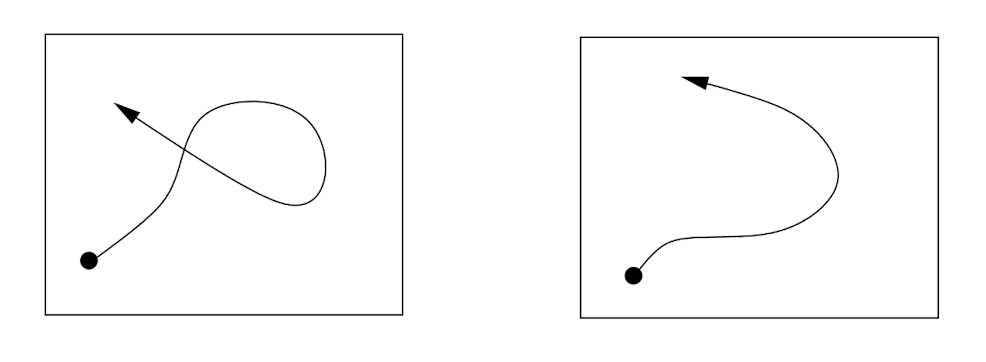
\includegraphics[scale = 0.5]{phase}	
\centering
\vspace{0.1in}
\caption{Moto nello spazio delle configurazioni (sinistra) e nello spazio delle fasi (destra)}
\end{figure}


\subsection{Equazioni di Hamilton}
Vogliamo determinare una funzione definita sullo spazio delle fasi che descriva in modo univoco l'evoluzione rispetto a $q_i$ e $p_i$. Questo vuol dire che deve essere in funzione di $q_i$ e $p_i$ e debba contenere la stessa informazione data dalla Lagrangiana $\mathcal{L}(\underline{q}(t),\underline{\dot q}(t),t)$. Per farlo utilizziamo una trasformazione di coordinate definita trasformazione di Legendre.
Definiamo la funzione \textbf{Hamiltoniana} come la trasformata di Legendre della Lagrangiana rispetto alle variabili $\dot q_i$.
\begin{equation}
	H\left(q_i, p_i, t\right)=\sum_{i=1}^n p_i \dot{q}_i-L\left(q_i, \dot{q}_i, t\right)
\end{equation}
Dove l'ipotesi fondamentale \`{e} data dal fatto che dalla relazione (5.2) sia possibile determinare $\dot q_i(q_i,p_i,t)$, ovvero si richiede che la trasformazione di coordinate sia invertibile rispetto alle $\dot q_i$.\newline
La variazione di H \`{e} data da:
\begin{equation}
	d H=\left(d p_i \dot{q}_i+p_i d \dot{q}_i\right)-\left(\frac{\partial L}{\partial q_i} d q_i+\frac{\partial L}{\partial \dot{q}_i} d \dot{q}_i+\frac{\partial L}{\partial t} d t\right)
\end{equation}
\begin{equation*}
	=d p_i \dot{q}_i-\frac{\partial L}{\partial q_i} d q_i-\frac{\partial L}{\partial t} d t
\end{equation*}
Il differenziale di sinistra pu\`{o} essere riscritto come
\begin{equation}
	d H=\frac{\partial H}{\partial q_i} d q_i+\frac{\partial H}{\partial p_i} d p_i+\frac{\partial H}{\partial t} d t
\end{equation}
l'uguaglianza ottenuta ci permetter di definire un sistema di equazione di 2n equazioni differenziali del primo ordine che prendono il nome di \textbf{equazioni di Hamilton}
\begin{align}
	\begin{cases}
	\dot{p}_i  =-\frac{\partial H}{\partial q_i} \\
	\dot{q}_i  =\frac{\partial H}{\partial p_i} \\
	\frac{\partial L}{\partial t} = -\frac{\partial H}{\partial t}
	\end{cases}	
\end{align}	
Rispetto alle equazioni di E-L che definivano un sistema di N equazioni differenziali del secondo ordine
abbiamo costruito un sistema di 2N equazioni differenziali del primo ordine.\newline
Si nota che la funzione di Hamilton coincide con l'energia del sistema E($q,\dot q, t$) data dall'\textbf{integrale di Jacobi} per la Lagrangiana di un sistema.

\subsection{Esempi}

\subsubsection{1) Particella in un potenziale}

Consideriamo una particella che si muove in un potenziale centrale in uno spazio a 3 dimensioni. La Lagrangiana sar\`{a} data da
\begin{equation*}
	L = \dfrac{1}{2}|\underline{\dot x}|^2 - U(\underline{x})
\end{equation*}
Le equazioni di E-L associate sono:
\begin{align}
	\begin{cases}
		\ddot x_1 = -\dfrac{dU(\underline{x})}{dx_1} \\
		\quad \;\,\vdots \\
		\ddot x_n = -\dfrac{dU(\underline{x})}{dx_n} 
	\end{cases}
	\quad \iff \quad
	\begin{cases}
		\dot x_1 = y_1 \\
		\dot y_1 = -\frac{dU(\underline{x})}{dx_i}\\
		\quad \;\,\vdots \\
		\dot x_n = y_n \\
		\dot y_n = - \frac{dU(\underline{x})}{dx_n}
	\end{cases}
\end{align}	
Usando la relazione (5.2) e (5.4) otteniamo
\begin{equation*}
	p=\frac{\partial \mathcal{L}}{\partial \dot{x}}=\dot{x} \quad \quad  \quad H=p \dot{x}-\mathcal{L}(x, \dot{x}(x, p))
\end{equation*}
dunque la Hamiltoniana associata al sistema \`{e} data da 
\begin{equation*}
H=p^2-\frac{p^2}{2}+U(x)=\frac{p^2}{2}+U(x)	
\end{equation*}
usando le equazioni in (5.7) definiamo le equazioni di Hamilton del sistema dinamico 
\begin{align*}
	\begin{cases}
		\dot x_i=p_i \\
		\dot p_i=-U^{\prime}(\underline{x})
	\end{cases}
	\quad i = 1,...,n
\end{align*}
posto $y_i = p_i$ nelle equazioni in (5.8) si ha che le equazioni di Hamilton e di E-L sono equivalenti tra loro.

\subsubsection{2) Invertibilit\`{a} delle velocit\`{a} generalizzate}

La Lagrangiana di un sistema \`{e} data da
\begin{equation*}
	\mathcal{L}=\frac{1}{2} g(q) \dot{q}^2-U(q)
\end{equation*}
dove g(q) \`{e} una funzione delle coordinate generalizzate e la quantit\`{a} di moto generalizzata \`{e} esprimibile come
\begin{equation*}
	p=g(q) \dot{q} \quad \text{dove} \quad g(q)>0 
\end{equation*}
di conseguenza la trasformazione di coordinate \`{e} invertibile, infatti
\begin{equation*}
	\dot q(q,p) = \dfrac{p}{g(q)}
\end{equation*}
e la Hamiltoniana associata al sistema pu\`{o} essere riscritta come
\begin{equation*}
	H = \dfrac{p^2}{2g(q)} + U(q)
\end{equation*}
dove le rispettive equazioni di Hamilton sono date da
\begin{align*}
	\begin{cases}
\frac{d u}{d t}=\frac{p}{g(q)} \\
 \frac{d}{d t} p=\frac{1}{2}\frac{g^{\prime}(q)}{g^2(q)} p^2-\frac{\partial}{\partial q} U \\
	\end{cases}
\end{align*}
\vspace{0.1in}

\begin{theorem}[Equivalenza Eq. E-L ed Hamilton ]
Le equazioni di Eulero-Lagrange sono equivalenti alle equazioni di Hamilton.
\end{theorem}

\begin{proof}
Partiamo da un Hamiltoniana definita rispetto ad un Lagrangiana indipendente dal tempo $\frac{\partial \mathcal{L}}{dt} = 0$ e consideriamo uno spazio delle configurazioni C in una sola dimensione. La variazione della funzione di Hamilton sar\`{a} descritta dal differenziale

\begin{equation*}
	d H(q, p, t)=\frac{\partial H}{\partial q} d q+\frac{\partial H}{\partial p} d p
\end{equation*}
\newline
ricordando che $\dot q (q,p,t)$ si ha che l'equazione precedente \`{e} equivalente a 
\begin{equation*}
	d(p \dot{q}-\mathcal{L}(q, \dot{q}, t))= pd\dot q +dp \dot q - \dfrac{\partial \mathcal{L}}{\partial q}dq - \dfrac{\partial \mathcal{L}}{\partial \dot q}d \dot q =
\end{equation*}
\begin{equation*}
	= pd\dot q +dp \dot q - \dfrac{\partial \mathcal{L}}{\partial q}dq - pd \dot q = \dot q dp - \dfrac{\partial \mathcal{L}}{\partial q}dq
\end{equation*}
\newline
dalle equazioni di E-L abbiamo che $\frac{d}{dt} \big [ \frac{\partial \mathcal{L}}{\partial \dot q} \big ] =\frac{\partial \mathcal{L}}{\partial  q} $ dunque l'uguaglianza precedente pu\`{o} essere riscritta come
\begin{equation*}
	=\dot q dp - \dfrac{d}{dt} \Big [\dfrac{\partial \mathcal{L}}{\partial \dot q} \Big ]dq = \dot q dp  + (- \dot p)dq
\end{equation*}
in conclusione otteniamo 
\begin{align*}
	\begin{cases}
	\dot{p}_i  =-\frac{\partial H}{\partial q_i} \\
	\dot{q}_i  =\frac{\partial H}{\partial p_i} \\
	\end{cases}
\end{align*}
\end{proof}

\begin{proof}
	Si consideri dim[C] $>1$ procediamo come nel caso in una dimensione definendo il differenziale dell'Hamiltoniana
\begin{equation*}
	d H=\sum_{j=1}^n \frac{\partial H}{\partial q_j} d q_j+\sum_{j=1}^n \frac{\partial H}{\partial p_j} d p_j+\frac{\partial H}{\partial t}
\end{equation*}
le j-sime equazioni possono essere riscritte come 
	\begin{alignat*}{2}
		\dfrac{\partial H}{\partial q_j}=\sum_i^n p_i \dfrac{\partial \dot{q}_i}{\partial q_j}-\dfrac{\partial \mathcal{L}}{\partial q_j}-\sum_{i=1}^n \dfrac{\partial \mathcal{L}}{\partial \dot{q}_j} \dfrac{\partial \dot{q}_i}{\partial q_j} = -\dfrac{\partial \mathcal{L}}{\partial q_j}+\underbrace{\sum_{i=1}^n \frac{\partial \dot{q}_i}{\partial q_j}\left[\frac{\partial \mathcal{L}}{\partial \dot{q}_i}-p_i\right]}_{=0} \\[0.05cm]
		\dfrac{\partial H}{\partial p_j}=\sum_i^n \dot{q}_i \dfrac{\partial p_i}{\partial p_j}+\sum_i^n p_i \dfrac{\partial \dot{q}_i}{\partial p_j}-\sum_i^n \dfrac{\partial \mathcal{L}}{\partial \dot{q}_i} \dfrac{\partial \dot{q}_i}{\partial p_j} = \dot{q}_j + \underbrace{\sum_i^n \frac{\partial \dot{q}_i}{\partial p_j}\left[\frac{\partial \mathcal{L}}{\partial \dot{q}_i}-p_i\right]}_{=0}\\[0.05cm]
		\dfrac{\partial H}{\partial t}=-\dfrac{\partial \mathcal{L}}{\partial t}-\sum_i^n \dfrac{\partial \mathcal{L}}{\partial \dot{q}_i} \dfrac{\partial \dot{q}_i}{\partial t}+\sum_i^n p_i \dfrac{\partial \dot{q}_i}{\partial t} = -\dfrac{\partial \mathcal{L}}{\partial t}+\underbrace{\sum_{i=1}^n \frac{\partial \dot{q}_i}{\partial t}\left[\dfrac{\partial \mathcal{L}}{\partial \dot{q}_i}-p_i\right]}_{=0}
	\end{alignat*}
di conseguenza si ottiene un sistema di 2N equazioni differenziali al primo ordine.
\end{proof}

\subsection{Leggi di conservazione}

\begin{lemma}
Se $\frac{\partial H}{\partial t} = 0$ allora H \`{e} una costante del moto
\end{lemma}

\begin{lemma}
	Se una coordinata trascurabile q non compare nella Lagrangiana allora per costruzione non apparte nemmeno nella Hamiltoniana. I momenti coniugati $p_q$ associati a q sono conservati.
\end{lemma}

\subsection{Momenti coniugati rispetto alla trasformazione di Legendre}

\begin{theorem}
Se la Lagrangiana di un sistema \`{e} rappresentabile come
\begin{equation}
	\mathcal{L} = \frac{1}{2} \sum_{\alpha, \beta}  G_{\alpha, \beta}  \cdot \dot{q}_\alpha \;\dot{q}_\beta-U = \frac{1}{2} \langle \underline{\dot q},G \underline{\dot q}\rangle - \;U
\end{equation}
dove G(q) \`{e} una matrice simmetrica ed invertibile associata all'energia cinetica del sistema $\Rightarrow$ si ha che il vettore dei momenti coniugati e le velocit\`{a} generalizzate possono essere scritte come
\begin{equation}
	\underline{p} = G(\underline{q})\cdot \underline{\dot q} \quad \text{e} \quad \dot q = G^{-1}(p) \cdot \underline p
\end{equation}
\end{theorem}

\subsubsection{Esempio}
La trasformata di Legendre definita da una Lagrangiana della forma come in (5.9) \'{e} data da
\begin{align*}
	 p \dot{q}=\frac{1}{2}\left\langle\dot{q}, G_{\dot{q}}\right\rangle+U &=\\
	&=\left\langle p, G^{-1} p\right\rangle-\frac{1}{2}\left\langle G^{-1} p, G G^{-1} p\right\rangle+U=\\
	&=\left\langle p, G^{-1} p\right\rangle-\frac{1}{2}\left\langle p, G^{-1} p\right\rangle+U
\end{align*}
dunque la Hamiltoniana associata \`{e} data da 
\begin{equation*}
	H = \dfrac{1}{2}\left\langle p, G^{-1} p\right\rangle + U
\end{equation*}

\begin{remark}
Data una matrice simmetrica invertibile, l'inversa \`{e} ancora una matrice simmetrica e $(G^{-1})^T = (G^T)^{-1}$.
\end{remark}

\subsection{Formulazione variazionale delle equazioni di Hamilton}

Si \`{e} definita l'azione come 
\begin{equation*}
	S[q]=\int_{t_0}^{t_1} L\left(q_i, \dot{q}_i, t\right) d t
\end{equation*}
poich\`{e} Hamiltoniana e Lagrangiana sono legate dalla trasformata di Legendre possiamo invertire tale relazione per riscrivere il funzionale d'azione come 
\begin{equation}
	S[q]=\int_{t_0}^{t_1}\left(p_i \dot{q}_i-H\right) d t
\end{equation}
Applicando il teorema 5.2.8 andiamo ricercare i punti che rendono stazionaria l'azione
\begin{flalign*}
\delta S & =\int_{t_0}^{t_1}\left\{\delta p_i \dot{q}_i+p_i \delta \dot{q}_i-\frac{\partial H}{\partial p_i} \delta p_i-\frac{\partial H}{\partial q_i} \delta q_i\right\} d t \\[1.2em]
& =\int_{t_0}^{t_1}\left\{\left[\dot{q}_i-\frac{\partial H}{\partial p_i}\right] \delta p_i+\left[-\dot{p}_i-\frac{\partial H}{\partial q_i}\right] \delta q_i\right\} d t+\left[p_i \delta q_i\right]_{t_0}^{t_1}
\end{flalign*}
dove il termine $p_i\delta \dot{q_i}$ \`{e} stato integrato per parti, ovvero

\begin{equation*}
	\int_{t_0}^{t_1}p_i\delta \dot{q}_i \,dt = p_i\delta q_i \vert_{t_0}^{t_1} - \int_{t_0}^{t_1} \dot {p}_i \delta q \,dt
\end{equation*}
di conseguenza abbiamo che il differenziale d'azione S \`{e} nullo quando
\begin{equation*}
	\dot{q}_i=\frac{\partial H}{\partial p_i} \quad \text { e } \quad \dot{p}_i=-\frac{\partial H}{\partial q_i}
\end{equation*}
dobbiamo imporre alle condizioni al contorno che l'ultimo addendo dell'equazione sia nulla ovvero 
\begin{equation*}
	\delta q_i(t_0) = \delta q_i(t_1) = 0
\end{equation*}
Notare che imponendo tale condizione $\delta p_i$ sono libere di variare a piacimento, non rendendo simmetrico il formalismo. Volendo potremmo imporre la condizione anche sulle $\delta p_i$, ma cos\`{i} facendo restringeremmo ancora di pi\`{u} i cammini possibili.

\section{Parentesi di Poisson}

\begin{definition}
	Siano f(q,p) e g(q,p) due funzione definite sullo spazio delle fasi si definisce \textbf{parentesi di Poisson}
	\begin{equation}
		\{f, g\}=\frac{\partial f}{\partial q_i} \frac{\partial g}{\partial p_i}-\frac{\partial f}{\partial p_i} \frac{\partial g}{\partial q_i}
	\end{equation}
\end{definition}
\noindent Le parentesi di Poisson godono delle seguenti propriet\`{a}:
\begin{itemize}
	\item Antisimmetria: $\{f,g\}$ = $-\{g,f \}$
	\item Bilinearit\`{a}: $\{\alpha f+\beta g, h\}=\alpha\{f, h\}+\beta\{g, h\}$  per ogni $\alpha,beta \in \mathbb{R}$
	\item Regola di Leibniz: $\{f g, h\}=f\{g, h\}+\{f, h\} g$ che deriva dalla chain rule della differenziazione.
	\item Identit\`{a} di Jacobi: $\{f,\{g, h\}\}+\{g,\{h, f\}\}+\{h,\{f, g\}\}=0$
\end{itemize}

\begin{lemma}
	Si consideri il punto $(q_1,...,q_n,p_1,..,p_n)\in \mathcal{F} \times \mathbb{R}$ nello spazio delle fasi e la Hamiltoniana H che definisce le eq. del moto 
\begin{align*}
	\begin{cases}
	\dot{p}_i  =-\frac{\partial H}{\partial q_i} \\
	\dot{q}_i  =\frac{\partial H}{\partial p_i} \\
	\end{cases}	
\end{align*}	
data una grandezza fisica $F(q_1,...,q_n,p_1,...,p_n)$ definita sullo spazio delle fasi, la sua derivata totale(overo l'evoluzione temporale di posizioni e momenti) pu\`{o} essere scritta come 
\begin{equation}
	\dfrac{dF}{dt} = \Big \{F,H \Big\} + \dfrac{\partial F}{\partial t}
\end{equation}
\end{lemma}

\begin{proof}
\begin{align*}
\frac{d F}{d t} & = \sum_{i = 1}^N\frac{\partial F}{\partial p_i} \dot{p}_i+ \sum_{i=1}^N\frac{\partial f}{\partial q_i} \dot{q}_i+\frac{\partial F}{\partial t} \\[0.5em]
& = \sum_{i=1}^N \Big [\frac{\partial F}{\partial q_i} \frac{\partial H}{\partial p_i} -\frac{\partial F}{\partial p_i} \frac{\partial H}{\partial q_i} \Big ] + \frac{\partial F}{\partial t} \\[0.5em]
& =\{f, H\}+\frac{\partial f}{\partial t}
\end{align*}
\end{proof}
\noindent Con l'uso delle parentesi di Poisson dotiamo le variabili dinamiche che descrivono l'evoluzione di un sistema nella meccanica Hamiltoniana di una struttura algebrica. Utilizzando tale notazione le equazioni di Hamilton assumono una forma simmetrica tra le posizioni e i momenti coniugati.

\begin{align}
	\left\{\begin{array}{l}
		\dot{q_j}=\left\{q_j, H\right\} \\
		\dot{p_j}=\left\{p_j, H\right\}
	\end{array}\right.
	\quad j=1,...N
\end{align}
\vspace{0.1in}
\begin{definition}
	Si definisce costante del moto una funzione I definita sullo spazio delle fasi tale per cui
	\begin{equation}
		\Big \{ I,H \Big \}=0
	\end{equation}
	so dice che I ed H \textbf{commutano rispetto Poisson}. 
\end{definition}

\subsubsection{Esempio}

Si ipotizzi che $q_i$ sia una coordinata ignorabile (per esempio non compare in H) allora 
\begin{equation*}
	\Big \{ p_i,H \Big \} = 0
\end{equation*}
essa esprime la relazione tra coordinate ignorabili e le quantit\`{a} conservabili nel linguaggio delle parentesi di Poisson. 
\newline
\begin{remark}
	Se I e J sono costanti del moto allora $\{\{I,J\},H\} + \{I,\{J,H\}\} + \{\{I,H\},J\} = 0$ e dunque anche $\{I,J\}$ \`{e} una costante del moto. Si dice che le costanti del moto formano un algebra chiusa rispetto alle parentesi di Poisson.
\end{remark}

\section{Trasformazioni Canoniche}

Le equazioni di Hamilton possono essere riscritte in un modo che risultino pi\`{u} simmetriche. Definiamo il vettore $\vec{x} = (q_1,...,q_n,p_1,....,p_n)^T$ di dimensione 2N e la matrice J di grandezza $2N \times 2N$,

\begin{align}
\mathcal{J}=\left[\begin{array}{ccccc}
0 & 1 & & & 0 \\
-1 & 0 & & & \\
& & \ddots & & \\
& & & 0 & 1 \\
0 & & & -1 & 0
\end{array}\right]
= \left[\begin{array}{cc}
		\underline{0} & I_n \\
		-I_n & \underline{0}
\end{array} \right]
\end{align}
dove $I_n$ \`{e} la matrice identica di dimensione $n \times n$. Nella notazione compatta ogni entrata \`{e} una matrice $n \times n$. La matrice $\mathcal{J}$ \`{e} definita come la \textbf{matrice simplettica}. In questa notazione le equazioni di Hamilton possono essere riscritte come 
\begin{equation}
	\underline{\dot{x}} = \mathcal{J} \cdot \nabla_{\underline{x}} H
\end{equation}
In meccanica Lagrangiana si \`{e} visto come \`{e} possibile effettuare un cambio di coordinate da $q_i \rightarrow Q(q_i)$ senza cambiare la forma delle equazioni. Nella formulazione Hamiltoniana vogliamo estendere il concetto di trasformazione di coordinate per le posizioni $q_i$ e i momenti $p_i$ in un nuovo sistema $P_i$ e $Q_i$ per mezzo di un insieme di equazioni invertibili

\begin{align}
	\begin{array}{c}
		Q_i = Q_i(q,p,t)\\[0.5em]
		P_i = P_i(q,p,t)
	\end{array}	
\end{align}
dove le nuove coordinate sono funzione sia delle vecchie coordinate che anche dei momenti coniugati. Come nel caso Lagrangiano ci domandiamo quale classe di trasformazioni ci permetta di lasciare invariate le equazioni di Hamilton. Consideriamo una trasformazione
\begin{equation*}
	x_i \mapsto y_i(x)
\end{equation*}
applicando la relazione (5.20) si ha che 
\begin{equation*}
	\dot{y}_i = \sum_{j=1}^{2N}\dfrac{\partial y_i}{\partial x_j}\dot{x}_j = \sum_{j=1}^{2N}\dfrac{\partial y_i}{\partial x_j} \mathcal{J}_{jk} \dfrac{\partial H}{\partial y_l}\dfrac{\partial y_l}{\partial x_k}
\end{equation*}
in modo compatto pu\`{o} essere riscritto come

\begin{equation*}
	\dot{y} = (J \mathcal{J} J^T) \nabla_yH
\end{equation*}
dove J \`{e} la matrice Jacobiana associata alla trasformazione di coordinate. Le equazioni di Hamilton sono invarianti in forma rispetto allo Jacobiano di una trasformazione se J soddisfa le condizioni

\begin{equation}
	J\mathcal{J}J^T = \mathcal{J} \quad \Rightarrow \quad \frac{\partial y_i}{\partial x_j} \mathcal{J}_{j k} \frac{\partial y_l}{\partial x_k}=\mathcal{J}_{i l}
\end{equation}
\newline
Se lo Jacobiano J soddisfa l'equazione (5.22) viene definito \textbf{simplettico}.
 Un cambio di coordinate in cui Jacobiano risulta essere simplettico viene definito \textbf{trasformazione canonica}.
 \newline 
 Nei paragrafi successivi vedremo che esiste un metodo efficace per costruire trasformazioni canoniche usando le funzioni generatrici.
\newline
\begin{theorem}[\textbf{Teorema d'invarianza per le trasformazioni canoniche}]
Si consideri una trasformazione di coordinate 
\begin{equation}
	(q_1,...,q_n,p_1,....,p_n) \rightarrow (Q_1,...,Q_n,P_1,...,P_n)
\end{equation}
diciamo che una trasformazione \`{e} canonica se e soltanto se preserva le parentesi fondiamenti di Poisson
\begin{equation}
	\left\{Q_i, Q_j\right\}=\left\{P_i, P_j\right\}=0 \quad \text { e } \quad\left\{Q_i, P_j\right\}=\delta_{i j}
\end{equation}
inoltre gli elementi della matrice simplettica sono rappresentabili come
\begin{equation}
	\left [ \begin{array}{ccc}
		\{q_i,q_j\} & \vline & \{q_i,p_j\}\\[0.1in]
		\hline 
		\{p_i,q_j\} & \vline & \{p_i,p_j\}\\[0.1in]
	\end{array} \right ]
	= \left [ \begin{array}{ccc}
		\mathbb{O}_{n \times n} & \vline & \mathbb{I}_{n \times n}\\[0.1in]
		\hline 
		-\mathbb{I}_{n \times n} & \vline & \mathbb{O}_{n \times n}\\[0.1in]
	\end{array} \right ]
\end{equation}
\end{theorem}
\begin{proof}
Consideriamo le coordinate $(q_1,..,q_n,p_1,..,p_n)$ e le riscriviamo in unico vettore $\vec{x} = (x_1,...,x_{2n})$, dove $\{ x_{\alpha},x_{\beta} \} = \mathcal{J}_{\alpha \beta}$ per $\alpha,\beta =1,..,2n$ coincidono con le componenti della matrice simplettica. Applicando la trasformazione di coordinate (5.23) applichiamo lo stesso procedimento per le coordinate $(Q_1,..,Q_n,P_1,..,P_n)$ definendo $\vec{\mathcal{X}}=(X_1,...,X_{2n})$ dove ogni elemento del vettore \`{e} dipendente dalle coordinate di partenza $X_{\alpha}(x_1,...,x_{2n})$. Fissato $\alpha$ poich\`{e} le componenti di $\vec{\mathcal{X}}$ non sono esplicitamente dal tempo possiamo scrivere la loro evoluzione temporale come
\begin{equation}
\frac{d}{d t} X_\alpha=\left\{X_\alpha, H\right\}=\sum_{\beta=1}^n \frac{\partial X_\alpha}{\partial x_\beta} \mathcal{J}_{\alpha \beta} \frac{\partial H}{\partial x_\beta}
\end{equation}
La nuova Hamiltoniana $K(Q_1,...,Q_n,P_1,...,P_n)$ definita rispetto alle nuove coordinate della trasformazione descrive il medesimo sistema se 
\begin{equation}
K(Q, P)=H(q, p)+\frac{\partial F}{\partial t}
\end{equation}
Ipotizzando che F sia una funzione generatrice non dipendente esplicitamente dal tempo la relazione (5.27) diventa 
\begin{equation}
	K(Q_1,...,Q_n,P_1,...,P_n)=H(q_1,..,q_n,p_1,..,p_n)
\end{equation}
dunque possiamo riscrivere le derivate parziali della Hamiltoniana H in (5.26) nel seguente modo
\begin{equation}
	\frac{\partial H(\vec{x}(\vec{\mathcal{X}}))}{\partial x_{\alpha}} = \frac{\partial K(\vec{\mathcal{X}}(\vec{x}))}{\partial x_{\alpha}} = \sum_{\eta = 1}^{2n}\frac{\partial K}{\partial X_{\eta}}\;\frac{\partial X_{\eta}}{\partial x_{\alpha}}
\end{equation}
sostituendo nell'equazione (5.26) si ha che 
 \begin{align}
 	\frac{d}{d t} X_\alpha=\left\{X_\alpha, H\right\}=\sum_{\beta=1}^n \frac{\partial X_\alpha}{\partial x_\beta} \mathcal{J}_{\alpha \beta} \sum_{\eta = 1}^{2n}\frac{\partial K}{\partial X_{\eta}}\;\frac{\partial X_{\eta}}{\partial x_{\alpha}} = \\[0.1in]
 	= \sum_{\eta=1}^{2 n}\left[\sum_{\beta=1}^{2 n} \frac{\partial X_\alpha}{\partial x_\beta} \mathbb{J}_{\beta \alpha} \frac{\partial X_\eta}{\partial x_\alpha}\right] \frac{\partial K}{\partial X_\eta} = \sum_{\eta=1}^{2 n}\left\{X_{\alpha}, X_\eta\right\} \frac{\partial K}{\partial X_\eta}
 \end{align}
 Se $\left\{X_{\alpha}, X_\eta\right\} = \mathcal{J}_{\alpha \eta}$ la trasformazione preserva la forma delle equazioni di Hamilton
\begin{equation}
\left\{\begin{array}{l}
\dot{Q}_j=\frac{\partial K}{\partial P_j} \\[0.1in]
\dot{P}_j=-\frac{\partial K}{\partial Q_j}
\end{array}\right \} \quad j=1,....,n
\end{equation}
e quindi la trasformazione \`{e} canonica. Viceversa ipotizziamo che la trasformazione sia canonica allora le componenti della matrice $\mathcal{J}$ coincidono con le parentesi di Poisson e dunque 
\begin{equation}
\frac{d}{d t} X_\alpha=\sum_\eta \mathcal{J}_{\alpha \eta} \frac{\partial K}{\partial X_\eta}
\end{equation} 
e dunque preserva la forma delle equazioni di Hamilton.

\end{proof}
\subsection{Funzioni generatrici per la trasformazioni canoniche} 



Nel capitolo di meccanica Lagrangiana si \`{e} visto come due descrizioni diverse tra loro dello stesso sistema fisico sono equivalenti se le rispettive Lagrangiane che lo descrivono differiscono tra loro per una derivata totale del tipo $\frac{d F(q,t)}{dt}$. \newline

\begin{theorem}[\textbf{Equivalenza equazioni E-L}]
	Siano $\tilde{L} (Q,\dot{Q},t)$ la Lagrangiana del sistema rispetto a delle coordinate Q e $L(q,\dot{q},t)$la Lagrangiana rispetto ad un sistema in coordinate q, allora descrivono il medesimo sistema fisico se 
	\begin{equation}
		\tilde{L} (Q,\dot{Q},t) = \lambda L(q,\dot{q},t) - \dfrac{dF(q,Q,t)}{dt}
	\end{equation}
\end{theorem}
\begin{remark}
Il segno meno all'interno dell'equazione (5.24) \`{e} per convenzione. Inoltre solo per $\lambda = 1$ si rappresenta una trasformazione canonica.
\end{remark}

\begin{proof}
Utilizziamo la definizione di Azione integrando l'equazione (5.24)

\begin{equation*}
	S[q,Q]=\int_{t_1}^{t_2} \tilde{L} d t=\int_{t_1}^{t_2} L d t+F\left(q\left(t_1\right), Q\left(t_1\right), t_1\right)-F\left(q\left(t_2\right), Q\left(t_2\right), t_2\right) 
\end{equation*} 
Riscriviamo il funzionale d'azione come
\begin{equation*}
	\tilde{S} -S  = \int_{t_0}^{t_1} (\tilde{L} -L) \, dt =   F\left(q\left(t_1\right), Q\left(t_1\right), t_1\right)-F\left(q\left(t_2\right), Q\left(t_2\right), t_2\right) 
\end{equation*}
Consideriamo un incremento infinitesimo $\varepsilon$ nella direzione $\underline{h}$ avremo che la variazione del funzionale $\tilde{S}-S $ \`{e} pari a 

\begin{align*}
	&\delta(\tilde{S}-S) = \lim_{\varepsilon \rightarrow 0} (\tilde{S}-S)[q+\varepsilon h] - (\tilde S-S)[q]= & \\[0.1in]
	&\lim_{\varepsilon \rightarrow 0} F(q(t_{1})+\epsilon h)- F(q(t_{2})+ \varepsilon h) - F\left(q\left(t_1\right), t_1\right)+F\left(q\left(t_2\right), t_2\right)= 0& \\[0.1in]
	& \Rightarrow \delta \tilde{S} = \delta S
\end{align*}
Dunque le equazioni di E-L definite dalle due Lagrangiane sono le medesime.
\end{proof}

\begin{remark}
Anche se le due funzioni Lagrangiane sono diverse da loro descrivono il medesimo sistema dato che definiscono le stesse equazioni di Eulero-Lagrange. 
\end{remark}

La funzione F pu\`{o} essere usata partendo da una Lagrangiana per generarne una nuova, che fornisce una descrizione equivalente a quella di partenza del sistema fisico.\newline
Poich\`{e} la Hamiltoniana \`{e} esprimibile come trasformata di Legendre della Lagrangiana quanto espresso rispetto alle equazioni di E-L \`{e} estendibile alle equazioni di Hamilton.
\begin{equation}
	K = \dot{Q}P - \dot{q}p + H + \frac{dF(q,Q,t)}{dt}
\end{equation}
con la comparsa di termini in pi\`{u} e condizioni al contorno. Definendo la 1-forma differenziale
\begin{equation}
	dF =  pdq - PdQ + (K-H)dt
\end{equation}
\subsection{Cambi di coordinate}

Consideriamo di avere un sistema nelle coordinate (Q,P) e di voler passare alle coordinate (p,q) per farlo definiamo una funzione

\begin{align*}
	\begin{cases}
		Q = Q(q,p)\\
		P = P(q,p)\\
	\end{cases}
\end{align*}

Affinch\`{e} la trasformazione sia un cambio di coordinate deve essere invertibile, ovvero $det J \neq 0$ dove J \`{e} la matrice Jacobiana.

\begin{align}
J = 
\left [ \begin{array}{cc}
		\dfrac{\partial Q}{\partial q} & \dfrac{\partial Q}{\partial p} \\ [0.2in]
		\dfrac{\partial P}{\partial q} & \dfrac{\partial P}{\partial p} \\
	\end{array}\right ]
\end{align}
\newline

\noindent La matrice Jacobiana associata al cambio di coordinate \`{e} di fondamentale importanza in quanto le condizioni sulle sue componenti definiscono condizione necessaria e sufficiente affich\`{e} una funzione F sia una funzione generatrice di una trasformazione canonica, ovvero che le parentesi di Poisson siano preservate.

\subsection{Jacobiano e condizione di canonicit\`{a}}
\noindent Definiamo il passaggio di coordinate 

\begin{align*}
	\begin{cases}
		p = p(q,Q)\\
		P = P(q,Q)\\
	\end{cases}
\end{align*}
verifichiamo che le parentesi di Poisson siano preservate

\begin{equation}
	\{Q,P\} = \left(\frac{\partial P}{\partial p}\right)_q\left(\frac{\partial Q}{\partial q}\right)_p-\left(\frac{\partial P}{\partial q}\right)_p\left(\frac{\partial Q}{\partial p}\right)_q
\end{equation}
possiamo riscrivere alcuni addendi nel seguente modo

\begin{equation}
	\left(\frac{\partial P}{\partial p}\right)_q=\left(\frac{\partial P}{\partial Q}\right)_q\left(\frac{\partial Q}{\partial p}\right)_q
\end{equation}
e
\begin{equation*}
	\left(\frac{\partial P}{\partial q}\right)_p=\left(\frac{\partial P}{\partial q}\right)_Q+\left(\frac{\partial P}{\partial Q}\right)_q\left(\frac{\partial Q}{\partial q}\right)_p
\end{equation*}
sostituendo all'interno dell'espressione (5.28) della parentesi di Poisson possiamo riscriverla come

\begin{equation}
	\{Q,P\} = -\left(\frac{\partial Q}{\partial p}\right)_q\left(\frac{\partial P}{\partial q}\right)_Q = \left(\frac{\partial Q}{\partial p}\right)_q\left(\frac{\partial p}{\partial Q}\right)_q = 1
\end{equation}
Il passaggio 
\begin{equation*}
	\left(\frac{\partial P}{\partial q}\right)_Q = -\left (\frac{\partial p}{\partial Q}\right)_q
\end{equation*}
si \`{e} ottenuta come condizione di canonicit\`{a} dall'espressione (5.20) e l'inveritibilit\`{a} del cambio di coordinate.
\newline
Osservando la struttura della (5.28) e della (5.29) si ha che posto 
\begin{equation}
	\frac{\partial Q}{\partial p} = 0
\end{equation} 
elemento della matrice Jacobiana la parentesi di Poisson non viene preservata e dunque non si ottiene una trasformazione di coordinate che preserva la matrice simplettica.
Resta da determinare come tali informazioni si leghino alla scelta della funzione generatrice.

\subsection{Funzione generatrice di I specie}

Definiamo funzione generatrice del primo tipo una funzione $F_1$(q,Q,t) associata ad un cambio di coordinate
\begin{align*}
	\begin{cases}
		p = p(q,Q)\\
		P = P(q,Q)\\
	\end{cases}
\end{align*}
consideriamo la il differenziale totale associato alla funzione 

\begin{equation}
	\frac{d F(\mathbf{q}, \mathbf{Q}, t)}{d t}=\left[\frac{\partial F_1(\mathbf{q}, \mathbf{Q}, t)}{\partial \mathbf{q}} \cdot \dot{\mathbf{q}}+\frac{\partial F_1(\mathbf{q}, \mathbf{Q}, t)}{\partial \mathbf{Q}} \cdot \dot{\mathbf{Q}}\right]+\frac{\partial F_1(\mathbf{q}, \mathbf{Q}, t)}{\partial t}
\end{equation}
sostituendo nella relazione (5.26)
\begin{align*}
	&\left[\mathbf{p}-\frac{\partial F_1(\mathbf{q}, \mathbf{Q}, t)}{\partial \mathbf{q}}\right] \cdot \dot{\mathbf{q}}-H(\mathbf{q}, \mathbf{p}, t)= & \\[0.4cm]
	&=\left[\mathbf{P}+\frac{\partial F_1(\mathbf{q}, \mathbf{Q}, t)}{\partial \mathbf{Q}}\right] \cdot \dot{\mathbf{Q}}-K(\mathbf{Q}, \mathbf{P}, t)+\frac{\partial F_1(\mathbf{q}, \mathbf{Q}, t)}{\partial t}
\end{align*}
affinch\`{e} la Hamiltoniana nelle nuove coordinate descriva il medesimo sistema fisico e la trasformazione sia canonica si deve avere che 
\begin{equation}
	K(\mathbf{Q}, \mathbf{P}, t)=H(\mathbf{q}, \mathbf{p}, t)+\frac{\partial F_1(\mathbf{q}, \mathbf{Q}, t)}{\partial}
\end{equation}
di conseguenza si deve avere che 
\begin{equation}
	\begin{cases}
	\mathbf{p}=\frac{\partial F_1(\mathbf{q}, \mathbf{Q}, t)}{\partial \mathbf{q}} \\
	 \mathbf{P}=-\frac{\partial F_1(\mathbf{q}, \mathbf{Q}, t)}{\partial \mathbf{Q}}\\
	 K = H + \frac{\partial F_1}{\partial t}
	\end{cases}
\end{equation}
Condizione necessaria e sufficiente affinch\`{e} la trasformazione sia canonica \`{e}
\begin{equation}
	\frac{\partial Q}{\partial p} \neq  0
\end{equation}	
Inoltre si estende quanto discusso alla funzione $F_1(q,Q,t)$ affinch\`{e} sia una funzione generatrice, prendendo l'equazione (5.30) e sostituendo rispetto a (5.34)
\begin{equation}
	\{Q,P\} = -\left(\frac{\partial Q}{\partial p}\right)_q\left(\frac{\partial P}{\partial q}\right)_Q = \left(\frac{\partial Q}{\partial p}\right)_q \frac{\partial^2 F_1}{\partial q \partial Q } = 1
\end{equation}
\newline
Affinch\`{e} le parentesi di Poisson siano preservate \`{e} necessario che
\begin{equation}
	\frac{\partial^2 F_1}{\partial q \partial Q } \neq 0
\end{equation} 
\begin{remark}
Dunque dimostrare che la componente $J_{12}$ \`{e} della matrice Jacobiana \`{e} non nulla, per quanto discusso nella sezione precedente equivale a dimostrare che $F_1$ \`{e} una funzione generatrice del primo tipo. 	
\end{remark}

\subsection{Funzione generatrice del II tipo}

Procedendo come per le funzioni del primo tipo, definiamo una funzione $F = F_2(q,P,t) - QP $ associata alla trasformazione di coordinate 
\begin{equation}
\begin{cases}
	p = p(q,P)\\
	Q = Q(q,P)
\end{cases}
\end{equation}
il differenziale della funzione \`{e} dato da 
\begin{equation}
	dF_2 = pdq +QdP + (K-H)dt
\end{equation}
e 
\begin{equation}
	{dF_2(q,P,t)}= \frac{\partial F_2}{\partial q}dq +\frac{\partial F_2}{\partial P}dP + \frac{\partial F_2}{\partial t}dt
\end{equation}
di conseguenza le coordinate canoniche (5.38) possono essere riscritte come

\begin{align}
	\begin{cases}
		p = \frac{\partial F_2}{\partial q} \\
		Q = \frac{\partial F_2}{\partial P} \\
		K = H + \frac{\partial F_2}{\partial t}
	\end{cases}
\end{align}
Condizione necessaria e sufficiente affinch\`{e} una trasformazione canonica ammetta funzione generatrice di seconda specie \`{e}
\begin{equation}
	\frac{\partial P}{\partial p} \neq 0
\end{equation}
che per quanto discusso in precedenza equivale a porre una condizione su $F_2(q,P,t)$ del tipo

\begin{equation}
	\frac{\partial F_2(q,P,t)^2}{\partial q \partial P} \neq 0
\end{equation}

\subsection{Funzione generatrice del III tipo}

Definiamo una funzione del terzo tipo $F = F_3(p,Q,t) + qp$ associata ad una trasformazione canonica 
\begin{align}
	\begin{cases}
		q = q(p,Q)\\
		P = p(p,Q)
	\end{cases}
\end{align}

il differenziale della funzione F \`{e} dato da

\begin{equation}
	dF_3 = -q d p-P d Q+(K-H) d t
\end{equation}	
e 
\begin{equation}
	dF_3 = \frac{\partial F_3}{\partial p} d p+\frac{\partial F_3}{\partial Q}dQ +\frac{\partial F_3}{\partial t} d t
\end{equation}
le coordinate della trasformazione canonica associata assumono la forma 
\begin{align}
	\begin{cases}
		q = - \frac{\partial F_3}{\partial p}\\
		P = - \frac{\partial F_3}{\partial Q}\\
		K = H + \frac{\partial F_3}{\partial t}
	\end{cases} 
\end{align}
Condizione necessaria e sufficiente affinch\`{e} le parentesi di Poisson siano preservate \`{e}
\begin{equation}
	\frac{\partial Q}{\partial q} \neq 0
\end{equation}
che equivale a imporre una condizione sulla funzione $F_3$ 
\begin{equation}
	\frac{\partial F_3(p,Q,t)}{\partial p \partial Q } \neq 0
\end{equation}

\subsection{Funzione generatrice del IV tipo}

Definiamo funzione generatrice del quarto tipo una funzione $F = F_4(p,P,t) + qp - QP $ associata alla trasformazione canonica
\begin{align}
	\begin{cases}
		q = q(p,P)\\
		Q = Q(p,P)
	\end{cases}
\end{align}
studiando il differenziale della funzione generatrice otteniamo 
\begin{equation}
	dF_4 = \frac{\partial F_4}{\partial p} d p+\frac{\partial F_4}{\partial P}dP +\frac{\partial F_4}{\partial t} d t
\end{equation}
e 
\begin{equation}
	dF_4 = -qdp + QdP + (K-H)dt  
\end{equation}
e di conseguenza la trasformazione (5.50) \`{e} uguale a  
\begin{equation}
	q = -\frac{\partial F_4}{\partial p}\\
	Q = \frac{\partial F_4}{\partial P}
	K = H + \frac{\partial F_4}{\partial t}
\end{equation}

Affinch\`{e} la trasformazione preservi le parentesi di Poisson deve valere la seguente condizione sugli elementi della matrice Jacobiana associata 
\begin{equation}
	\frac{\partial P}{\partial q} \neq 0
\end{equation}
ed estesa alla funzione generatrice $F_4$ diventa 
\begin{equation}
	\frac{\partial F_4}{ \partial p \partial P}\neq 0
\end{equation}

\renewcommand\arraystretch{1.6}
\begin{align*}
\begin{array}{|c|c|}
\hline \text { Funzione generatrice } & \text { Trasformazione  } \\
\hline \hline F_1(q, Q, t) & p_i=\frac{\partial F_1}{\partial q_i}, P_i=-\frac{\partial F_1}{\partial Q_i} \\
\hline F_2(q, P, t) - QP & p_i=\frac{\partial F_2}{\partial q_i}, Q_i=\frac{\partial F_2}{\partial P_i} \\
\hline F_3(p, Q, t) + qp & q_i=-\frac{\partial F_3}{\partial p_i}, P_i=-\frac{\partial F_3}{\partial Q_i} \\
\hline F_4(p, P, t) +qp -QP & q_i=-\frac{\partial F_4}{\partial p_i}, Q_i=\frac{\partial F_4}{\partial P_i} \\
\hline
\end{array}
\end{align*}
\newline
\begin{remark}
	Quanto discusso per due variabili \`{e} generalmente estendibile a pi\`{u} dimensioni.
\end{remark}

\section{Trasformazioni di Contatto}

Si consideri un sistema Hamiltoniano con in coordinate $(\vec{q},\vec{p})$ definiamo la trasformazione con pi\`{u} di un grado di libert\`{a} 
\begin{align}
	\left\{\begin{array}{l}
Q_k=Q_k\left(q_1, \ldots, q_d\right) \\
P_k=\sum_{j=1}^{d} A_{k j}\left(q_1, \ldots q_d\right)p_j
\end{array}\right.
\end{align}
allora valgono i seguenti risultati:
\begin{enumerate}
	\item La trasformazione \`{e} canonica se e soltanto se 
	\begin{equation}
		J_{(q,Q)} = ({A^{-1}})^T
	\end{equation}
	\item La funzione generatrice \`{e} del secondo tipo e ha la forma
	\begin{equation}
		F_2(q,P) = \sum_{j=1}^d Q_j(\vec{q})P_j
	\end{equation}
\end{enumerate}
trasformazioni di questo tipo in cui $P_k$ \`{e} esprimibile come combinazione lineare delle $\vec{p}$ \`{e} e le $Q_k$ dipendono solo da $\vec{q}$ vengono chiamate \textbf{trasformazioni di contatto}.
\begin{proof}
La matrice Jacobiana associata alla trasformazione di coordinate \`{e} della forma 
\begin{align}
J = 
\left [\begin{array}{ccc}
	J_{(q,Q)} & \quad \vline & \underline{0}\\
	\hline 
	\star & \quad \vline &A(\vec{q})\\
\end{array}\right ]
\end{align} 
affinch\`{e} la trasformazione sia una trasformazione di coordinate \`{e} necessario che sia invertibile ovvero $detJ \neq 0$, il determinane della matrice  Jacobiania \`{e} dato da 
\begin{equation}
	detJ = det (J_{(q,Q)})det(A(\vec{q})) \neq 0
\end{equation}
ci\`{o} implica che $det(A(\vec{q})) \neq 0$, tale risultato coincide con la condizione necessaria e sufficiente affinch\`{e} la trasformazione ammetta una funzione generatrice del secondo tipo (inoltre $A(\vec{q})$ \`{e} invertibile).
Dati tali risultati possiamo riscrivere la trasformazione (5.56) come 
\begin{align}
	\begin{cases}
		Q_k = \frac{\partial F_2}{\partial P_k}\\
		p_k = \sum_{j=1}^{d} A^{-1}_{kj}(\vec{Q})P_j = \frac{\partial F_2}{\partial q_k} 
	\end{cases}
\end{align}
integrando il primo membro otteniamo la forma di $F_2$
\begin{equation}
	F_{2}^{k} = \int Q_kdP_k = Q_kP_k + G(\vec{q},\vec{P})
\end{equation}
risolvendo le prime d equazioni avremo che 
\begin{equation}
	F_2 = \sum_{j=1}^{d} Q_jP_j + \phi(\vec{q})
\end{equation}
sostituendo rispetto al secondo membro della (5.62) abbiamo che 
\begin{equation}
	\sum_{j=1}^{d} A^{-1}_{kj}(\vec{Q})P_j = \sum_{j=1}^d \frac{\partial Q_j}{\partial q_k}P_j + \frac{\partial \phi(\vec {q})}{\partial q_k}  
\end{equation}
per avere che $\phi (\vec{q})$ sia una soluzione comune a tutte le equazioni \`{e} necessario che sia una funzione costante e dunque $\frac{\partial \phi(\vec {q})}{\partial q_k} = 0$, di conseguenza la (5.64) diventa 
\begin{equation}
	\sum_{j=1}^{d} A^{-1}_{kj}(\vec{Q})P_j = \sum_{j=1}^d\frac{\partial Q_j}{\partial q_k}P_j 
\end{equation}
da (5.65) abbiamo che 
\begin{equation}
	A^{-1}_{kj}(\vec{Q}) = \frac{\partial Q_j}{\partial q_k}
\end{equation}
ovvero gli elementi della matrice inversa di A coincidono con gli elementi della matrice Jacobiana trasposta, la (5.65) pu\`{o} essere riscritta in modo compatto come
\begin{equation}
	A^{-1} \cdot \vec{P} = J_{(q,Q)}^{T} \cdot \vec{P}
\end{equation}
di conseguenza poich\`{e} l'operazione di trasposizione gode della propriet\`{a} d'idempotenza si ha 
\begin{equation}
	J_{(q,Q)} = (A^{-1})^{T}
\end{equation}
Inoltre dato che $\frac{\partial \phi(\vec {q})}{\partial q_k} = 0$ la (5.63) diventa 
\begin{equation}
	F_2 = \sum_{j=1}^{d} Q_jP_j
\end{equation}
\end{proof}

\section{Hamiltoniane esplicitamente dipendenti dal tempo ed estensione dello spazio delle fasi}

Consideriamo un sistema dinamico descritto da una funzione Hamiltoniana esplicitamente dipendente dal tempo 
\begin{equation}
	H = H(q,p,t) \quad \Big (\frac{\partial H}{\partial t} \neq 0 \Big )
\end{equation}
le rispettive equazioni di Hamilton saranno date da
\begin{align}
	\begin{cases}
		\dot{q_j} = \frac{\partial H}{\partial p_j}\\
		\dot{p_j} = - \frac{\partial H}{\partial q_j}\\
		\frac{dH}{dt} = \frac{\partial H}{\partial t}
	\end{cases} \quad j = 1,...n
\end{align}
le grandezze fisiche associate saranno definite sullo \textbf{spazio delle fasi} ovvero saranno  funzioni esplicitamente dipendenti dal tempo e della forma
\begin{equation}
	G(q,p,t) : \mathcal{I} \times \mathbb{R^+} \rightarrow \mathbb{R}
\end{equation}
dalla relazione (5.16) sappiamo che la derivata totale di una funzione G \`{e} data da 
\begin{equation}
	\frac{d G}{dt} = \Big \{ G,H \Big \} + \frac{\partial G}{\partial t}
\end{equation}
che descrive l'evoluzione di G(q,p,t). \`{E} possibile definire uno \textbf{spazio delle fasi esteso} $\mathcal{I} \times \mathbb{R}^2_+$ introducendo due parametri (E,s) che ci permettono di riscrivere le equazioni di Hamilton esplicitamente dipendenti dal tempo in un nuovo sistema rispetto al quale sono indipendenti dalla variabile temporale.
Per le nuove variabili introdotte (E,s) deve valere che 
\begin{align}
	\{E,s \} = 1 \quad \{E,q_j \} = \{E,p_j\} = 0 \\
	\{s,q_j \} = \{s,p_j\} = 0 
\end{align}
Dai risultati precedenti si possono definire i due seguenti teoremi:

\begin{theorem} Data un Hamiltoniana H(q,p,t) esplicitamente dipendente dal tempo, dati due parametri (E,s) si pu\`{o} estendere la Hamiltoniana H sullo spazio delle fasi esteso definendola come 
\begin{equation}
	\mathcal{H}(q,p,E,s) = H(q,p,s)-E
\end{equation} 
Allora la nuova Hamiltoniana ottenuta e le rispettive equazioni di Hamilton non dipendono pi\`{u} esplicitamente dal tempo.
\end{theorem}
\begin{proof}
Data $\mathcal{H}$(q,p,E,s) = H(q,p,s) - E le rispettive equazioni di Hamilton si scrivono come
\begin{align}
	\begin{cases}
		\dot{q_j} = \frac{\partial H(q,p,s)}{\partial p_j}\\
		\dot{p_j} = - \frac{\partial H(q,p,s)}{\partial q_j}\\
		\frac{dE}{dt} = \frac{\partial H(q,p,s)}{\partial s}\\
		\frac{ds}{dt} = -\frac{\partial H(q,p,s)}{\partial E}
	\end{cases} \quad j = 1,...n
\end{align}
le equazioni di Hamilto date dal sistema (5.77) rispetto alla Hamiltonina $\mathcal{H}$ non dipendono esplicitamente dal tempo. Inoltre $\frac{ds}{dt} = -1$ che integrando si ottiene $s \equiv t$, usando tale risultato abbiamo che le equazioni di Hamilton nello spazio esteso diventano
\begin{align}
	\begin{cases}
		\dot{q_j} = \frac{\partial H(q,p,s)}{\partial p_j}\\
		\dot{p_j} = - \frac{\partial H(q,p,s)}{\partial q_j}\\
		\frac{dE}{dt} = \frac{dH(q,p,t)}{dt} =  \frac{\partial H(q,p,t)}{\partial t}
	\end{cases}
\end{align}
in questo modo si riottiene il sistema di equazioni esplicitamente dipendente dal tempo.

\end{proof}

\begin{theorem}
	Consideriamo una grandezza fisica 
	\begin{equation*}
		G(q,p,t) : \mathcal{I} \times \mathbb{R}^+ \rightarrow \mathbb{R}
	\end{equation*}
	definita sullo spazio delle fasi, se introduciamo dei parametri (E,s) tale grandezza \`{e} definibile sullo spazio delle fasi esteso come
	\begin{equation}
		\mathcal{G}(q,p,s): \mathcal{I} \times \mathbb{R}^2_+ \rightarrow \mathbb{R}
	\end{equation}
eliminando la dipendenza esplicita dal tempo, allora l'evoluto dinamico di tale quantit\`{a} rispetto ai nuovi parametri sar\`{a} dato da 
\begin{equation}
	\frac{d\mathcal{G}}{dt} = \{\mathcal{G},\mathcal{H} \}
\end{equation}
\end{theorem}
\begin{proof}
Sviluppiamo la parentesi di Poisson 
\begin{equation}
	\{\mathcal{G},\mathcal{H} \} = \sum_{j=1}^n \frac{\partial \mathcal{G}}{\partial q_j} \frac{\partial \mathcal{H}}{\partial p_j}-\frac{\partial \mathcal{G}}{\partial p_j} \frac{\partial \mathcal{H}}{\partial q_j}+\frac{\partial \mathcal{G}}{\partial E} \frac{\partial \mathcal{H}}{\partial s}-\frac{\partial \mathcal{G}}{\partial s} \frac{\partial \mathcal{H}}{\partial E}
\end{equation}
dalla dimostrazione del teorema precedente sappiamo che $\frac{\partial \mathcal{H}}{\partial E} = -1$ e dunque $s \equiv t$ inoltre $\frac{\partial \mathcal{G}}{\partial E} = 0 $, e per le relazioni del sistema (5.77) ci si riconduce all'espressione  
\begin{equation*}
	\frac{d G}{dt} = \Big \{ G,H \Big \} + \frac{\partial G}{\partial t}
\end{equation*}
\end{proof}

\section{Risoluzione di un problema di Cauchy con l'utilizzo delle trasformazioni canoniche e le equazioni di Hamilton}

Consideriamo il seguente problema di Cauchy rispetto alle coordinate (q,p)
\begin{align}
	\begin{cases}
		\dot{q} = \frac{p}{q^4}\\
		\dot{p} = \frac{2p^2}{q^4}-q^2\\
		q(0) = 1\\
		p(0) = 0 \\
	\end{cases}
\end{align}
Determininiano la Hamiltoniana H(q,p) associata al problema di Cauchy, ovvero imponiamo che 
\begin{align}
	\begin{cases}
		\dot{q} = \frac{p}{q^4} = \frac{\partial H}{\partial p}\\
		\dot{p} = \frac{2p^2}{q^4}-q^2 = -\frac{\partial H}{\partial q}\\
	\end{cases}
\end{align}
 integrando la prima equazione rispetto dp abbiamo
 \begin{equation}
 	H = \frac{p^2}{2q^4} + G(q)
 \end{equation}
 sostituendo in nella seconda relazione in (5.83)
 \begin{equation}
	\frac{2p^2}{q^4}-q^2 = \frac{2p^2}{q^4} - G^{\prime}(q)
 \end{equation}
 e dunque 
 \begin{equation}
G(q) = \int_{0}^{q} q^2dq = \frac{q^3}{3} 	
 \end{equation}
ed in conclusione sostituendo in (5.84) la Hamiltoniana H \`{e} della forma 
\begin{equation}
	H(q,p) = \frac{1}{2}\,\frac{p^2}{q^4} + \frac{q^3}{3} 
\end{equation}
Possiamo interpretare la relazione (5.87) come l'energia totale del sistema, data dalla somma dell'energia cinetica e dell'energia potenziale
\begin{equation}
	H(q,p) = T(q,p) + U(q)
\end{equation}
La struttura di H ci suggerisce di applicare una trasformazione canonica di contatto, ovvero della forma 
\begin{equation}
	\begin{cases}
		Q = U(q)\\
		P = P(q,p)\\
	\end{cases} \iff
	\begin{cases}
		Q = \frac{q^3}{3} \\
		P = P(q,P)\\
	\end{cases}
\end{equation}
Affinch\`{e} la trasformazione sia canonica \`{e} necessario che le parentesi di Poisson siano preservate
\begin{equation*}
	\{Q,P\} = \frac{\partial Q}{\partial q}\frac{\partial P}{\partial p}= q^2 \frac{\partial P}{\partial p} = 1 \Rightarrow \frac{\partial P}{\partial p} = \frac{1}{q^2}
\end{equation*}
integrando si ha 
\begin{equation}
	P(q,p) = \frac{p}{q^2}
\end{equation}
dunque la trasformazione di contatto \`{e} data da
\begin{equation}
\begin{cases}
		Q = \frac{q^3}{3} \\
		P = \frac{p}{q^2}\\
\end{cases}
\end{equation}
Determiniamo la nuova Hamiltonia K(Q,P) rispetto alle nuove coordinate definendo la trasformazione canonica inversa e andando a sostituire nella Hamiltoniana H(q,p) determinata nell'equazione (5.87)
\begin{equation}
	\begin{cases}
		q = [3Q]^{1/3}\\
		p = P[3Q]^{3/2}\\
	\end{cases}
\end{equation}
dunque K(Q,P) \`{e} uguale ad 
\begin{equation}
	K(Q,P) = \frac{1}{2}\;P^2 + Q
\end{equation}
definiamo le equazioni di Hamilton rispetto alla Hamiltoniana K
\begin{equation}
	\begin{cases}
		\dot{Q} = \frac{\partial K}{\partial P}=P\\
		\dot{P} = - \frac{\partial K}{\partial Q} = -1
	\end{cases}
\end{equation}
il problema di Cauchy nelle nuove coordinate \`{e} dato da 
\begin{equation}
	\begin{cases}
		\dot{Q} = \frac{\partial K}{\partial P}=P\\
		\dot{P} = - \frac{\partial K}{\partial Q} = -1\\
		Q(0) = \frac{1}{3}\\
		P(0) = 0
	\end{cases}
\end{equation}
integrando le equazioni rispetto al tempo ed effettuando le opportune sostituzioni 
\begin{equation}
	\begin{cases}
		Q = Q(0) + \int_{0}^{t} Pdt = \frac{1}{3} - \int_{0}^{t} tdt = \frac{1}{3} - \frac{1}{2} \,t^2\\
		P = -t 
	\end{cases}
\end{equation}
sostituendo nella (5.92) otteniamo la soluzione rispetto al problema di Cauchy di partenza dato da (5.82)
\begin{equation}
\begin{cases}
	q = \left[1-\frac{3}{2} t^2\right]^{1 / 3} \\
	p = -t\left[1-\frac{3}{2} t^2\right]^{2 / 3}\\
	\end{cases}
\end{equation}

\section{Trasformazioni Canoniche Infinitesime}

Consideriamo la trasformazione identit\`{a} delle coordiante, questa sar\`{a} data da una funzione generatrice 

\begin{equation}
	F(q,P) = qP
\end{equation}
 dove avremo 
 \begin{align}
 	\begin{cases}
 		p = \frac{\partial F}{\partial q} = P \\
 		Q = \frac{\partial F}{\partial P } = q \\
 	\end{cases}
 \end{align}
e quindi una mappa dove $q \rightarrow Q$ e $p \rightarrow P$.\newline
Ipotizziamo di perturbare in modo infinitesimo e lineare la trasformazione di identit\`{a} definendo
\begin{align}
	\begin{cases}
		Q = q + \varepsilon f(q,p) + o(\varepsilon)\\
		P = p + \varepsilon g(q,p) + o(\varepsilon)
	\end{cases}
\end{align}
trasformazioni di questo tipo prendono il nome di \textbf{trasformazioni infinitesime}. 

\subsection{Condizione di canoncit\`{a} per le trasformazioni infinitesime }
La domanda che ci poniamo \`{e} quale forma devono avere f e g affinch\'{e} (5.100) sia una trasformazione canonica, ovvero lasci invariato il problema in forma; per rispondere a tale domanda verifichiamo la condizione di canonicit\`{a}, ovvero che le parentesi di Poisson sia preservate.

\begin{theorem}
	Data una trasformazione di coordinate $(q,p) \rightarrow (Q,P)$ della forma 
	\begin{align}
	\begin{cases}
		Q = q + \varepsilon f(q,p) + o(\varepsilon)\\
		P = p + \varepsilon g(q,p) + o(\varepsilon)
	\end{cases}
\end{align}
tale trasformazione \`{e} canonica se e soltanto se le parentesi di Poisson sono preservate.
\end{theorem}
\begin{equation}
	\Big \{  Q,P \Big \} =  1 + o(\varepsilon) \quad \Big \{  P,Q \Big \} = -1 + o(\varepsilon)
\end{equation}

\begin{equation*}
	\Big \{  Q,Q \Big \} = 0 + o(\varepsilon) \quad \Big \{  P,P \Big \} = 0 +  o(\varepsilon)
\end{equation*}

\begin{proof}
\begin{align*}
	\Big \{  Q,P \Big \} = \{q+\varepsilon f(q, p)+o(\varepsilon), p+\varepsilon g(q, p)+o(\varepsilon)\}= &\\
	= \{q, p\}+\varepsilon[\{q, g(q, p)\}+\{f(q, p), p\}]+0(\varepsilon) 
\end{align*}
dove $\{q, p\} = 1$ mentre il secondo addendo fornisce la condizione
\begin{equation}
	\{q, g\}+\{f, p\}=0 \quad \text{ovvero} \quad \frac{\partial g}{\partial p}+\frac{\partial f}{\partial q}=0
\end{equation}
Se consideriamo un insieme semplicemente connesso nel piano delle fasi (q,p), tale condizione coincide con l'esistenza di una funzione F(q,p) tale che 
\begin{align}
	\begin{cases}
		f= \frac{\partial F(q,p)}{\partial p} \\
		g= - \frac{\partial  F(q,p)}{\partial q}\\
	\end{cases}
\end{align}
che rende la trasformazione canonica e soddisfa dunque le condizioni posto in (5.102).

\end{proof}
\noindent Dal risultato ottenuto dalla dimostrazione precedente possiamo definire una \textbf{trasformazione canonica infinitesima} come
\begin{align}
	\begin{cases}
		Q = q + \varepsilon \,\frac{\partial F(q,p)}{\partial p} + o(\varepsilon)\\
		P = p - \varepsilon  \,\frac{\partial  F(q,p)}{\partial q}+ o(\varepsilon)
	\end{cases}
\end{align}

\subsection{Famiglia di trasformazioni canoniche ad un parametro}
Se consideriamo la trasformazione (5.105) rispetto al parametro $\varepsilon$ questa appartiene alle trasformazioni canoniche ad 1 parametro e la funzione F coincide con la Hamiltoniana del sistema
\begin{align}
	\begin{cases}
		\frac{dQ_{\varepsilon}}{d \varepsilon} = \frac{\partial F}{ \partial p}\\
		\frac{dP_{\varepsilon}}{d \varepsilon} = - \frac{\partial F}{ \partial q}\\
	\end{cases}
\end{align}
\begin{definition}
	Un gruppo ad un parametro di trasformazioni canoniche \`{e} un gruppo di simmetria rispetto H se 
	\begin{equation}
		H(Q_{\varepsilon},P_{\varepsilon}) = H(q,p) \Rightarrow \frac{d}{d \varepsilon}\Big [H(Q_{\varepsilon},P_{\varepsilon}) - H(q,p) \Big ] = 0
	\end{equation}
	ovvero la Hamiltoniana resta invariata rispetto alla trasformazione.
\end{definition}

\begin{definition}
	Una famiglia ad un parametro di trasformazioni canoniche \`{e} di simmetria per la Hamiltoninana H se e solo se $\{H,F\} = 0$.
\end{definition}

\begin{definition}
	Consideriamo una famiglia di trasformazioni canoniche ad un parametro, parametrizzate da $s \in \mathbb{R}$ nello spazio delle configurazioni M allora valgono le seguenti propriet\`{a}:
	\begin{enumerate}
		\item f(q,p,0) \`{e} l'identit\`{a}
		\item $f^{-1}$(q,p,s) = f(q,p,-s) 
		\item f(f(q,p,$s_1$),$s_2$) = f(q,p,$s_1 + s_2$)
		\item $\forall$ q,p fissati, f \`{e} definibile rispetto ad $s \in \mathbb{R}$ ed esiste $\frac{\partial f}{\partial s}\vert_{s=0}$
	\end{enumerate}
\end{definition}

\subsection{Hamiltoniana di una trasformazione infinitesima}

Riscriviamo la Hamiltonina rispetto al nuovo sistema di coordinate definito dalla trasformazione canonica infinitesima (5.105)

\begin{align*}
	\frac{dH}{dt}= \lim_{\varepsilon \rightarrow 0} \frac{H(x+\epsilon f, p+\epsilon g)-H}{\varepsilon}=\, \lim_{\varepsilon \rightarrow 0} \frac{1}{\varepsilon} <\nabla H,\varepsilon\underline{h}>
= \\[0.2in] =\left(\frac{\partial H}{\partial q} f +\frac{\partial H}{\partial p} g\right) 
= \left(\frac{\partial H}{\partial q}\frac{\partial F}{\partial p}  -\frac{\partial H}{\partial p}\frac{\partial F}{ \partial q} \right)\equiv \Big \{ H,F \Big \}
\end{align*}
tale risultato \`{e} significativo in quanto se applichiamo le propriet\`{a} delle parentesi di Poisson si ha che 
\begin{align*}
	\frac{dF}{dt} = \frac{\partial J}{\partial q} \dot{q}+\frac{\partial J}{\partial p} \dot{p} = & \\
	= &\frac{\partial F}{\partial q } \frac{\partial H}{\partial p}-\frac{\partial F}{\partial p} \frac{\partial H}{\partial q} \equiv - \Big \{H,F \Big \}
\end{align*}
che ci descrive il cambiamento di F rispetto a moto di una particella, di conseguenza se si ha una funzione tale per cui $\{H,F\} = 0$, si ha che
\begin{enumerate}
	\item Dalla relazione precedente la Hamiltoniana resta invariata rispetto alla trasformazione di coordinate.
	\item F \`{e} una costante del moto
	\item L'evoluzione dinamica della Hamiltoniana pu\`{o} essere riscritta come trasformazione canonica.
\end{enumerate}

\section{Teorema di Noether per la meccanica Hamiltoniana}

\begin{theorem}[\textbf{Primo Teorema di Emmy Noether }]
	Sia F la funzione generatrice di una trasformazione canonica infinitesima essa \`{e} una simmetria per il sistema descritto dalle equazioni di Hamilton se e soltanto se \`{e} una costante del moto.
\end{theorem}

\begin{proof}
Consideriamo una trasformazione canonica infinitesima della forma
\begin{align*}
	\left\{\begin{array}{l}
Q=q+\varepsilon \frac{\partial f}{\partial p}+o(\varepsilon) \\
P=p-\varepsilon \frac{\partial f}{\partial q}+o(\varepsilon)
\end{array}\right.
\end{align*}
e sviluppiamo al primo ordine la Hamiltoniana definita rispetto alle nuove coordinate (Q,P)
\begin{align*}
H(Q, P) & =H\left(q+\varepsilon \frac{\partial f}{\partial p}+o(\varepsilon), p+\varepsilon\left(-\frac{\partial f}{\partial q}\right)+o(\varepsilon)\right)= \\[0.1in]
& =H(q, p)+\varepsilon\left[\frac{\partial H}{\partial q} \frac{\partial f}{\partial p}-\frac{\partial H}{\partial p} \frac{\partial f}{\partial q}\right]+o(\varepsilon)= \\[0.1in]
& =H(q, p)+\varepsilon \{ H, f\}+o(\varepsilon)
\end{align*}
La trasformazione canonica infinitesima definita \`{e} una simmetria per la Hamiltoniana se e soltanto se $\{ H,f \} = 0$ e quindi f lascia invariata H. Poich\`{e} le parentesi di Poisson godono della propriet\`{a} di antisimmetria $\{f,H \} = 0$ si ha che H lascia invariata f e dunque si conclude che f \`{e} una costante del moto per la Hamiltoniana H.
	
\end{proof}

\section{Teoria di Hamilton-Jacobi}

Si \`{e} visto che se la Hamiltoniana si conserva (ovvero non dipende esplicitamente dal tempo), allora le equazioni del Hamilton che rappresentano un sistema di equazioni differenziali si possono risolvere con una opportuna trasformazione che conduce ad un sistema di coordinate tutte cicliche e rispetto alle quali la soluzione del problema \`{e} immediata; altrimenti si pu\`{o} cercarcare una particolare trasformazione canonica che porti dal sistema di coordinate e momenti (q,p) all'instante t , in un sistema in cui le grandezze sono costanti. Per questi tipi di relazione la trasformazione che lega le coordinate vecchie a quelle nuove \`{e} la soluzione del problema meccanico
\begin{equation}
	\begin{aligned}
& q=q\left(q_0, p_0, t\right) \\
& p=p\left(q_0, p_0, t\right)
\end{aligned}
\end{equation}
che legano le coordinate e i momenti in funzione dei valori iniziali e del tempo.\newline
Scopo di questa sezione \`{e} determinare la forma di questa particolare trasformazione canonica.

\subsection{Equazione di Hamilton-Jacobi per la funzione principale di Hamilton}

Definiamo con K la Hamiltoniana rispetto alla trasformazione delle coordinate vogliamo che questa sia costante nel tempo, tale condizione di traduce nell'imporre che K sia identicamente nulla in modo tale che le equazioni di Hamilton rispetto alla funzione K nel nuovo sistema di coordinate siano
\begin{align}
	\begin{cases}
\frac{\partial K}{\partial P_i} & =\dot{Q}_i=0 \\
-\frac{\partial K}{\partial Q_i} & =\dot{P}_i=0
\end{cases}
\end{align}
inoltre la nuova Hamiltoniana K deve descrivere il medesimo sistema fisico descritto dalla funzione H definita rispetto le coordinate di partenza e dunque in accordo ai principi variazionali deve valere la relazione 
\begin{equation}
	K = H + \frac{\partial F}{\partial t}
\end{equation}
imponendo che K = 0 l'equazione (5.110) si traduce nella condizione 
\begin{equation}
	H(q,p,t) + \frac{\partial F}{\partial t} = 0
\end{equation}
La forma pi\`{u} semplice che pu\`{o} assumere F \`{e} che sia funzione delle vecchie coordinate $q_i$, dei nuovi momenti $P_i$ e del tempo. Una funzione di questo tipo coincide con una funzione generatrice di seconda specie $F_2(q,P)$ per una trasformazione canonica 
\begin{align*}
	\begin{cases}
		p_i = \frac{\partial F_2}{\partial q_i}\\
		Q_i = \frac{\partial F_2}{\partial P_i}
	\end{cases}
	\quad j = 1,...n
\end{align*}
dalla relazione definita dal primo elemento $p_i = \frac{\partial F_2}{\partial q_i}$ si pu\`{o} riscrivere l'equazione (5.111) come

\begin{equation}
	H\left(q_1, \ldots, q_n ; \frac{\partial F_2}{\partial q_1}, \ldots, \frac{\partial F_2}{\partial q_n} ; t\right)+\frac{\partial F_2}{\partial t}=0
\end{equation}
\newline
tale equazione \`{e} nota con il nome di \textbf{equazione di Hamilton-Jacobi}, ed \`{e}, per la funzione generatrice, un'equazione differenziale alle derivate parziali nelle (n+1) variabili $q_1,...,q_n,t$. La soluzione dell'equazione (5.112) viene indicata con S e prende il nome di \textbf{funzione principale di Hamilton}.\newline

\begin{remark}
	\`{E} È noto che trovare la soluzione generale di una equazione alle derivate parziali come quella di H-J è un problema di gran lunga pi\`{u} complicato che trovare la soluzione generale di un sistema di equazioni differenziali ordinarie (come le equazioni Hamiltoniane). Quindi pu\`{o} sembrare che l'idea di Jacobi sia solo formale e di poca utilit\`{a} pratica; in realt\`{a}
il fatto cruciale \`{e} che l'equazione di H-J pu\`{o} essere vista come una equazione alle derivate parziali per una funzione S(q,P,t), dove i momenti generalizzati nelle nuove coordinate sono considerati costanti come richiesto in (5.109).
\end{remark}

\subsubsection{Esempio}
Consideriamo la Hamiltoniana di un oscillatore armonico 

\begin{equation*}
	H=\frac{1}{2 m} p^2+\frac{k}{2} q^2
\end{equation*}
l'equazione di Hamilton-Jacobi associata, ipotizzando una soluzione della forma S(q,P,t) si scrive come 
\begin{equation*}
	\frac{1}{2 m}\left[\frac{\partial S}{\partial q}\right]^2+\frac{k}{2} q^2+\frac{\partial S}{\partial t}=0
\end{equation*}

\begin{definition}
	Se si ha un problema mono-dimensionale, ovvero si ha un solo parametro $\alpha=P$ si definisce \textbf{integrale completo} delle equazione di Hamilton-Jacobi una famiglia ad un parametro di soluzioni S(q,$P =\alpha$,t) tali per cui si ha che 
	\begin{equation*}
		\frac{\partial^2 S}{\partial P \partial q} \neq 0
	\end{equation*}
ovvero si richiede che la trasformazione di coordinate preservi la matrice simplettica e dunque S sia una funzione generatrice di seconda specie. \newline
Tale definizione si estende al caso in pi\`{u} imponendo la condizione
\begin{equation*}
	det\Big [ \frac{\partial^2 S}{\partial q_j \partial P_k}\Big ] \neq 0
\end{equation*}
\end{definition}

\subsection{Significato fisico della funzione principale di Hamilton}

Si consideri la derivata totale della funzione principale di Hamilton S(q,P,t) questa \`{e} data da 
\begin{equation}
	\frac{d S}{d t}= \sum_{i = 1}^{n-1}\frac{\partial S}{\partial q_i} \dot{q}_i+\frac{\partial S}{\partial t}
\end{equation}
dove si \`{e} sfruttato il fatto che i momenti $P_i$ sono costanti del tempo. Tale equazione sfruttando la relazione (5.112) pu\`{o} essere riscritta come 

\begin{equation}
	\frac{d S}{d t}= \sum_{i=1}^{n-1}p_i \dot{q}_i-H=L
\end{equation}
dunque la funzione principale di Hamilton differisce dall'integrale temporale indefinito della Lagrangiana per una costante 
\begin{equation}
	S = \int Ldt + C
\end{equation}

\subsection{Funzione caratteristica di Hamilton}

Se la Hamiltonina non dipende esplicitamente dal tempo, la funzione principale di Hamilton su pu\`{o} scrivere come
\begin{equation}
	S(q,\alpha,t) = W(q,\alpha) - \alpha t
\end{equation}

dove $W(q,\alpha)$ prende il nome di \textbf{funzione caratteristica di Hamilton}. Il significato fisico di W si comprende dalla sua derivata totale rispetto al tempo
\begin{equation}
	\frac{dW}{dt} =  \sum_{i=1}^{n-1}\frac{\partial W}{\partial q_i}\dot{q}_i
\end{equation}
sostituendo la (5.116) nella equazione (5.112) e confrontando il risultato con la (5.117) si ha che 
\begin{equation}
	p_i = \frac{\partial W}{\partial q_i}  \quad i = 1,...,n
\end{equation}
e quindi 
\begin{equation}
	\frac{dW}{dt} = \sum_{i=1}^{n-1}p_i\dot{q}_i
\end{equation}
integrando si ottiene 
\begin{equation}
	W = \sum_{i=1}^{n-1} \int p_idq_i
\end{equation}
ovvero l'azione abbreviata. \newline
L'equazione di Hamilton-Jacobi assume quella che viene definita una forma ristretta
\begin{equation}
	H(q_i,\frac{\partial W}{\partial q_i}) = \alpha_1
\end{equation}
che non contiene pi\`{u} il tempo esplicitamente.Una delle costanti d'integrazione e precisamente $\alpha_1$ deve essere uguale al valore costante di H. Si pu\`{o} dimostra che W genera a sua volta una trasformazione con propriet\`{a} diverse da quelle ottenute da S. \newline
\noindent Si consideri una trasformazione canonica in cui i nuovi momenti siano tutti costanti del moto $\alpha_i$ e in particolare $\alpha_1$  rappresenta la costante del moto H. Se indichiamo con W(q,P) la funzione generatrice di questa trasformazione, allora le equazioni saranno
\begin{align}
	\begin{cases}
		p_i = \frac{\partial W}{\partial q_i}\\
		Q_i = \frac{\partial W}{\partial P_i} = \frac{\partial W}{\partial \alpha_i}
	\end{cases}
	\quad i = 1,...,n
\end{align}
La condizione che permette di determinare W \`{e} l'imposizione che 
\begin{equation*}
	H(q_i,p_i) = \alpha_1
\end{equation*}
che sostituendo nell'equazione di Hamilton si traduce nell'equazione differenziale alle derivate parziali
\begin{equation}
	H \Big (q_i,\frac{\partial W}{\partial q_i} \Big ) = \alpha_1
\end{equation}
Poich\`{e} W non dipende esplicitamente dal tempo l'Hamiltoniana nuova e quella rispetto alle vecchie coordinate coincidono e dunque $K = \alpha_1$. \textit{la funzione caratteristica di Hamilton W genera una trasformazione canonica in cui tutte le nuove coordinate sono cicliche}. Poich\`{e} H \`{e} una costante del moto le equazioni di Hamilton coincidono con (5.109) rispetto a K e dunque una trasformazione di questo tipo risolve il problema meccanico. 
Le equazioni canoniche di $P_i$ si limitano a sottolineare che i momenti coniugati alle coordinate cicliche sono costanti 
\begin{equation*}
	\dot{P}_i=-\frac{\partial K}{\partial Q_i}=0 \quad P_i=\alpha_i \quad i = 1,..,n
\end{equation*}
e le equazioni del di $\dot{Q}_i$ sono 
\begin{equation}
\dot{Q}_i=\frac{\partial K}{\partial \alpha_i}= \begin{cases}=1 & i=1 \\ =0 & i \neq 1\end{cases}
\end{equation}
che ha soluzione 
\begin{equation}
\begin{aligned}
& Q_1=t+\beta_1 \equiv \frac{\partial W}{\partial \alpha_1} \\[0.3in]
& Q_i=\beta_i \equiv \frac{\partial W}{\partial \alpha_i} \quad i \neq 1
\end{aligned}
\end{equation}
La dipendenza di W dalle vecchie coordinate $q_i$ si ricava risolvendo l'equazione differenziale alle derivate parziali (5.123).\newline
\\
Non \`{e} sempre necessario che $\alpha_1$ e le costanti d'integrazione di W siano i nuovi momenti canonici costanti. A volte \`{e} pi\`{u} comodo scegliere come momenti trasformati un insieme di n funzioni indipendenti dalle $\alpha_i$. Indichiamo tali funzioni come $\gamma_i$. Le equazioni del moto per $\dot{Q}_i$ diventano
\begin{equation}
	\dot{Q}_i = - \frac{\partial K}{\partial \gamma_i} = v_i
\end{equation}
dove $v_i(\gamma_i)$. In questo caso tutte le nuove coordinate sono funzioni lineari del tempo
\begin{equation}
Q_i=v_i t+\beta_i
\end{equation}

\section{Separazione delle variabili per l'equazione di Hamilton-Jacobi}

In certe condizioni \`{e} possibile separare le variabili nell'equazione di Hamilton-Jacobi e in tale caso la soluzione di riduce alle quadrature. Il metodo di Hamilton-Jacobi si rivela utile dal punto di vista del calcolo solo quando questa separazione \`{e} possibile. Una coordinata $q_j$ si dice \textbf{separabile} nell'equazione di H-J se la funzione principale di Hamilton pu\`{o} essere divisa nella somma di due parti in cui una dipende solo dalla coordinata $q_j$ e l'altra ne \`{e} indipendente. Per comodit\`{a} di notazione ipotizziamo sia $q_1$ allora la funzione principale affich\`{e} sia separabile deve essere della forma
\begin{equation}
\begin{aligned}
S\left(q_1, \ldots, q_n ; \alpha_1, \ldots, \alpha_n ; t\right) & =S_1\left(q_1 ; \alpha_1, \ldots, \alpha_n ; t\right)+ \\
& +S^{\prime}\left(q_2, \ldots, q_n ; \alpha_1, \ldots, \alpha_n ; t\right)
\end{aligned}
\end{equation}
Si dice che l'equazione di Hamilton-Jacobi \`{e} \textbf{completamente separabile} (o semplicemente separabile), se tutte le coordinate del problema sono separabili.
\begin{equation}
S=\sum_i S_i\left(q_i ; \alpha_1, \ldots, \alpha_\pi ; t\right)
\end{equation}
l'equazione di H-J si divider\`{a} in n equazioni del tipo
\begin{equation}
H_i\left(q_j ; \frac{\partial S_j}{\partial q_j} ; \alpha_1, \ldots, k_n ; t\right)+\frac{\partial S_j}{\partial t}=0
\end{equation}
Considerando quanto discuso nella sezione precedente, se la Hamiltoniana non dipende esplicitamente dal tempo, per ogni $S_i$ si ha 
\begin{equation}
S_i\left(q_j ; \alpha_1, \ldots, \alpha_n t\right)=W\left(q_j ; \alpha_1, \ldots, \alpha_n ; t\right)-\alpha_i t
\end{equation}
e possiamo scrivere le n equazioni di H-J in forma ristretta 
\begin{equation}
H_i\left(q_i ; \frac{\partial W_i}{\partial q_i} ; \alpha_1, \ldots, \alpha_n\right)=\alpha_i
\end{equation}
Le costanti $\alpha_i$ prendono il nome di \textbf{costanti di separazione}. Ciascuna coinvolge un solo $q_i$ corrispettivo e una sola derivata parziale corrispondente rispetto $W_i$. In questo modo si \`{e} costruito un sistema di equazioni differenziali ordinarie del primo ordine, e tale categoria di EDO sono sempre risolvibili per quadrature.

\subsection{Separazione delle variabili per un potenziale centrale nel piano}

Si consideri un Hamiltoniana della forma 
\begin{equation}
H=\frac{1}{2 m}\left[p^{2}_r+\frac{p^{2}_{\theta}}{r^2}\right]+U(r)
\end{equation}
Definiamo una funzione generatrice di seconda specie $S(r,\theta,P_1,P_2,t)$ soluzione dell'equazione di H-J, poich\`{e} la Hamiltoniana del sistema non dipende esplicitamente dal tempo possiamo separare la variabile del tempo da S e riscrivere la funzione rispetto alla funzione caratteristica W dipendente solo dalle coordinate generalizzate
\begin{equation}
S\left(r, \theta, P_1, P_2, t\right)=W(r, \theta) + G(t)
\end{equation}
posto
\begin{equation}
p_r=\frac{\partial S}{\partial r} \quad \text { e } \quad p_\theta=\frac{\partial S}{\partial \theta}
\end{equation}
sostituendo in (5.133)
\begin{equation}
\frac{1}{2 m}\left[\left(\frac{\partial W}{\partial r}\right)^2+\frac{1}{r^2}\left(\frac{\partial W}{\partial \theta}\right)^2\right]+U(r)=-\frac{d G}{d t}
\end{equation}
dove 
\begin{equation}
	G(t) = -P_1t = - \alpha_1t
\end{equation}
in questo (5.136) diventa l'equazione di H-J ristretta
\begin{equation}
\frac{1}{2 m}\left[\left(\frac{\partial W}{\partial r}\right)^2+\frac{1}{r^2}\left(\frac{\partial W}{\partial \theta}\right)^2\right]+U(r)= \alpha_1
\end{equation}
Ipotizzando che la funzione caratteristica sia ulteriormente separabile abbiamo che 
\begin{equation}
	W(r, \theta)=W_1(r)+W_2(\theta)
\end{equation}
in questo modo riscriviamo la (5.138) come 
\begin{equation}
\begin{aligned}
& r^2\left(\frac{d W_1}{d r}\right)^2+\left(\frac{d W_2}{d \theta}\right)^2+U(r) 2 m r^2=\alpha_1 2 m r^2 \\[0.2in]
& \left(\frac{d}{d \theta} W_2\right)^2=\alpha_{1}2 m r^2-U(r) 2 m r^2-r^2\left(\frac{d}{d r} W_1\right)^2
\end{aligned}
\end{equation}
le due grandezze si equivalgono solo se sono uguali ad una costante $\alpha_2 = P_2$ e quindi otteniamo un sistema di due EDO del primo ordine, risolvibili per quadrature.
\begin{equation}
\left\{\begin{array}{l}
\frac{d}{d \theta} W_2=P_2 \rightarrow W_2= \alpha_2 \theta \\
\alpha_1 2 m r^2-U(r) 2 m r^2-r^2\left(\frac{d}{d r} W_{1}\right)^2=\alpha_2
\end{array}\right.
\end{equation}
risolviamola seconda equazione per quadrature 
\begin{equation}
W_1=\int^r\left[2 m\left(\alpha_1-U(\tilde{r})\right)-\frac{\alpha_2}{2 m \tilde{r}^2}\right]^{1 / 2} d \tilde{r}
\end{equation}
in conclusione la funzione principale dell'equazione di H-J \`{e} 
\begin{equation}
	S = W(r,\theta) - P_1t = W_1(r) + \alpha_2 \theta - \alpha_1t
\end{equation}
Verifichiamo la condizione di completezza affinch\`{e} S sia un integrale completo, ovvero data la trasformazione di coordinate
\begin{equation}
\left\{\begin{array}{l}
P_1=\frac{\partial S}{\partial q_1} \quad Q_1=\frac{\partial S}{\partial P_1} \\
P_2=\frac{\partial S}{\partial q_2} \quad Q_2=\frac{\partial S}{\partial P_2}\\

\end{array}\right.
\end{equation}
La Jacobiana associata alla trasformazione sar\`{a} data da 
\begin{align}
\left [ \begin{array}{ccccc}
	\phantom{''''''''''''''''''''''} & \phantom{} & \vline & \phantom{} & \phantom{}\\
	\phantom{} & \phantom{} & \vline & \phantom{} & \phantom{}\\
	\hline
	\phantom{} & \phantom{} & \vline & \frac{\partial S}{\partial P_1 \partial r} & \frac{\partial S}{\partial P_2 \partial r} \\
	\phantom{} & \phantom{} & \vline & \frac{\partial S}{\partial P_1 \partial \theta} & \frac{\partial S}{\partial P_2 \partial \theta} \\
\end{array}
\right ]
\end{align}
e si deve avere che il determinante della sotto matrice in (5.145) \`{e} diverso da zero.

\section{Problema ristretto dei tre corpi}
\subsection{Problema dei due corpi}
Consideriamo 2 punti materiali nello spazio di massa $m_1$ e $m_2$, che esercitano una forza conservativa di tipo gravitazionale tra loro. 
Definiamo la distanza reciproca tra i due punti e la posizione del centro di massa(baricentro)
\begin{equation}
\left\{\begin{array}{l}
\vec{x}=\frac{m_1 \vec{r}_2+m_2 \vec{r}_2}{M} \quad \text{dove} \quad M = \sum_{i=1}^{2}m_{i} \\
\vec{r}=\vec{r_2}-\vec{r_1}
\end{array}\right.
\end{equation}
La Lagrangiana del sistema \`{e} data da 
\begin{equation}
	\mathcal{L} = \frac{1}{2}m_{1}|\dot{\underline{r}}_1|^2 + \frac{1}{2}m_{2}|\dot{\underline{r}}_2|^2 - \frac{Gm_1m_2}{|\vec{r}_2 - \vec{r}_1|}
\end{equation}
possiamo riscrivere tale equazione come 
\begin{equation}
	\mathcal{L} = \frac{M}{2}|\dot{\underline{x}}|^2 + \boxed{\frac{1}{2}\mu |\dot{\underline{r}}|^2 - \frac{G m_1 m_2}{|\vec{r}|}} \quad \text{con} \quad \mu = \frac{m_1m_2}{m_1 + m_2}
\end{equation}
dove la componente del box dell'equazione (5.158) prende il nome di \textbf{problema ristretto}. La Lagrangiana in (5.156) \`{e} un problema a 6 g.d.l. e dunque se lo riscriviamo rispetto alle equazione di E-L si hanno 12 equazioni per la descrizione dello stato dinamico. Per questo motivo studiamo il problema ristretto che ha 3 g.d.l. e 5 integrali primi e le seguenti costanti del moto
\begin{enumerate}
	\item Energia
	\item Momento Lineare totale
	\item Momento angolare totale
	\item Vettore di Runge-Lenz
\end{enumerate} 
Se si \`{e} in un piano e si ha un integrale primo, si ha che le traiettorie percorse da un punto materiale sono curve chiuse. Nello spazio le traiettorie sono superfici, e se si hanno 2 punti materiali il cammino seguito sar\`{a} dato dall'intersezione delle superfici e dunque curve nello spazio.\newline
\noindent Per un potenziale Kepleriano le traiettorie descritte sono limitate alle coniche, ovvero ellissi, parabole ed iperboli. La terza legge di Keplero ci dice che il rapporto tra il cubo del semiasse maggiore e il quadrato del periodo dell'orbita \`{e} costante per tutti i corpi che appartengono alla traiettoria
\begin{equation}
	\frac{a^3}{T^2} = \frac{G(m_1+m_2)}{4 \pi^2}
\end{equation}
\subsection{Problema dei tre corpi ristretto}
Il problema dei 3 corpi generico \`{e} pi\`{u} complesso in quanto si hanno meno costanti del moto ed insorgono moti caotici. Per questo motivo si studia il problema dei tre corpi ristretto, ovvero si assume che 
\begin{equation}
	\frac{m_3}{m_1} << 1 \quad \frac{m_3}{m_2} << 1 \quad \text{e} \quad m_2 < m_1
\end{equation}
Consideriamo un sistema Terra, Luna e satellite, in questo caso la presenza di un satellite (massa $m_3$) non altra l'interazione tra i due corpi principali dati dalla Terra e la Luna. Per semplificare ulteriormente il problema si suppone che i moto del satellite sia sul piano individuato dai corpi principali e che essi si muovano in orbite circolari. Prendiamo periodo del moto circolare dei pianeti $T = 2 \pi$ ovvero $\omega = 1$. Poniamo 
\begin{equation*}
	\mu = \frac{m_2}{M} \quad \text{e} \quad 1-\mu
\end{equation*}
rispettivamente la massa del corpo $P_2$ e del corpo $P_1$.\newline
\begin{wrapfigure}{l}{0.5\textwidth}
  \begin{center}
    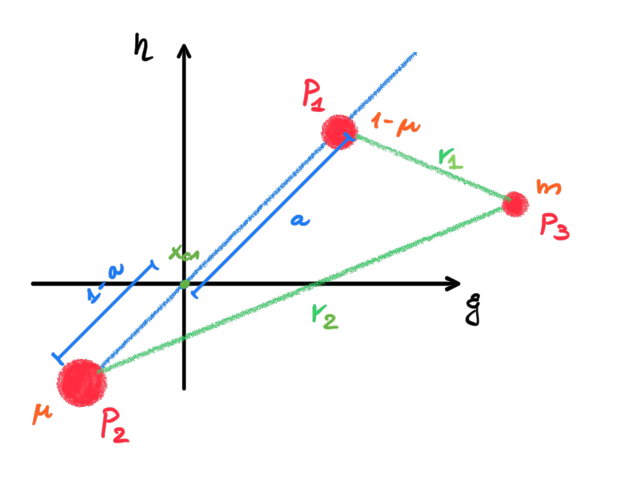
\includegraphics[width=0.5\textwidth]{3body}
  \end{center}
\end{wrapfigure}
\noindent Definiamo un sistema di coordinate la cui origine coincide con la posizione del centro di massa dei corpi  $P_1$ e $P_2$ di conseguenza in tutti gli istanti di tempo i due punti di trovano sulla retta congiungente, poich\`{e} si muovono relativamente al baricentro. Se osserviamo il sistema esternamente i due pianeti ruotano con $\omega = 1 $ e dunque la loro posizione dipende esplicitamente dal tempo.
La Lagrangiana del sistema \`{e} data dal sistema 

\begin{equation}
	\mathcal{L} = \frac{1}{2}m \Big [(\dot{\xi}^2 +\dot{\eta}^2) + \Big (\frac{1-\mu}{|\vec{r}_1|}- \frac{\mu}{|\vec{r}_2|} \Big ) \Big]
\end{equation}
\begin{wrapfigure}[7]{r}{0.4\textwidth}
    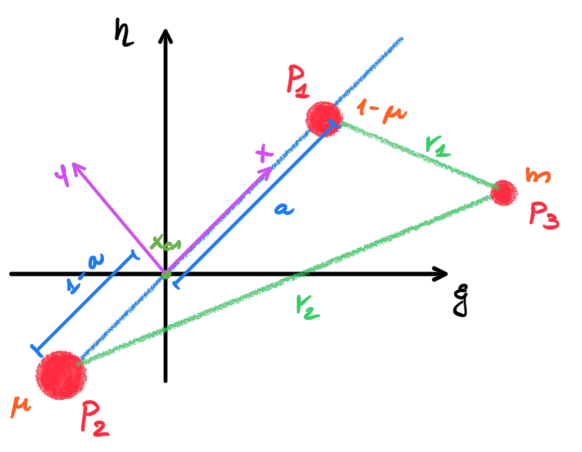
\includegraphics[width=0.4\textwidth]{relative}
\end{wrapfigure}

dove abbiamo ipotizzato il contributo al potenziale del corpo $P_3$ trascurabile e i punti $P_1$ e $P_2$ vincolati. Definiamo un sistema di riferimento S(x,y) solidale con i due pianeti $P_1$ e $P_2$. L'evoluzione dinamica di $P_3$ \`{e} data dall'applicazione della matrice di rotazione alle coordinate del punto rispetto al sistema comovente con i due pianeti.
\begin{equation}
\left [ \begin{array}{c}
\xi\\
\eta\\
\end{array} \right ] =
\left [ \begin{array}{cc}
cos(t) & -sin(t)\\
sin(t) & cos(t) \\
\end{array} \right ]
\left [ \begin{array}{c}
x\\
y\\
\end{array} \right ] =
\left\{\begin{array}{l}
\xi=x \cos t-y \sin t \\
\eta=x \sin t+y \cos t
\end{array}\right.
\end{equation}
Nel nuovo sistema la distanza del punto $P_3$ dagli altri due corpi non dipende pi\`{u} dal tempo.
\begin{figure}[!ht]
\centering
\begin{minipage}{0.5\textwidth}
  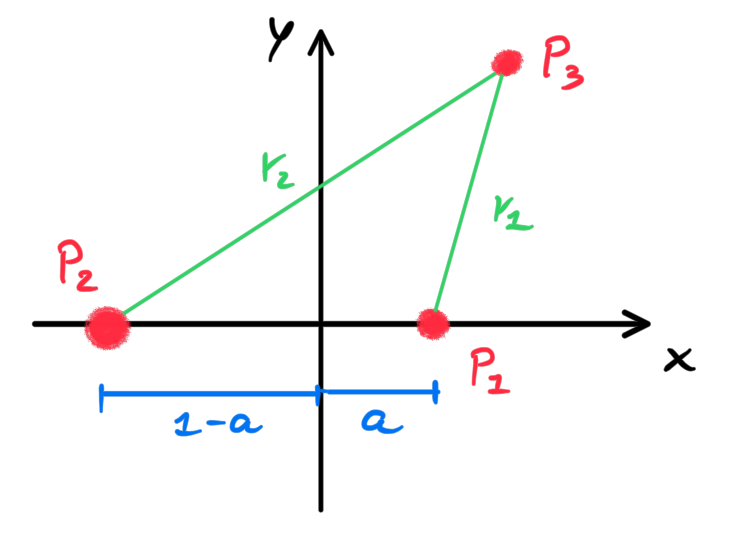
\includegraphics[width=1\linewidth]{plane}
\end{minipage}%
\begin{minipage}{.5\textwidth}
\begin{align}
	\begin{cases}
		\dot{\xi}^2 = (\dot{x} \cos t-x \sin t-\dot{y} \sin t-y \cos t)^2 = \\
		\dot{\eta}^2 =(\dot{x} \sin t+x \cos t+\dot{y} \cos t-y \sin t)^2 = 
	\end{cases}
\end{align}
\end{minipage}
\end{figure}
\vspace{-0.5in}
\begin{align*}
	\begin{cases}
		= \dot{x}^2 + x^2 +\dot{y}^2 + y^2 - 2\dot{x}y\\
		= \dot{x}^2 + x^2 +\dot{y}^2 + y^2 + 2\dot{x}y\\
	\end{cases}
\end{align*}
La Lagrangiana del sistema posto in rotazione \`{e} data da 
\begin{equation*}
	\mathcal{L} = \frac{1}{2}(\dot{x}-y)^2+\frac{1}{2}(\dot{y}-x)^2 + \frac{(1-\mu)}{\left[(x-a)^2+y^2\right]^{1 / 2}}+\frac{ \mu}{\left[(x+1-a)^2+y^2\right]^{1 / 2}} = 
\end{equation*}
\begin{equation}
	=\frac{1}{2}\left(\dot{x}^2+\dot{y}^2\right)-\underbrace{(\dot{x} y-\dot{y} x)}_{\text {Forza di Coriolis }}+\underbrace{\frac{1}{2}\left(x^2+y^2\right)}_{\text {Forza centrifuga }}+U_{g}
\end{equation}
I termini in pi\`{u} che compaiono sono dovuti al fatto che il riferimento \`{e} non inerziale. Procediamo a definire la Hamiltoniana del sistema effettuando la trasformata di Legendre della Lagrangiana. Associamo ai momenti e le velocit\`{a} generalizzate le seguenti grandezze
\begin{equation}
\begin{array}{ll}
p_x=\frac{\partial \mathcal{L}}{\partial x}=\dot{x}-y & \dot{x}= p_x+y \\
p_y=\frac{\partial \mathcal{L}}{\partial y}=\dot{y}+x & \dot{y}= p_y-x
\end{array}
\end{equation}
e dunque la Hamiltoniana del sistema \`{e} data da 
\begin{equation}
\begin{aligned}
H(p_x, p_y,\dot{x},\dot{y}) & =p_x \dot{x}+p_y \dot{y}-\mathcal{L}= \\[0.1in]
& =\frac{1}{2} p_x^2+p_y^2+y p_x-x p_y+\frac{1-\mu}{\left|r_1\right|}+\frac{\mu}{\left|r_2\right|}
\end{aligned}
\end{equation}
le equazioni di Hamilton rispetto alla Hamiltoniana H sono 
\begin{equation}
\left\{\begin{array}{l}
\dot{x}=p_x+y \\
\dot{y}=p_y-x \\
\dot{p}_x=-\frac{\partial H}{\partial x}= 
p_y-\frac{(1-\mu)(x-\mu)}{r_1^3}-\frac{\mu(1-\mu+x)}{r_2^3}\\
\dot{p}_y=-\frac{\partial H}{\partial y}= 
-p_x-y\left[\frac{(1-\mu)}{r_1^3}+\frac{\mu}{r_2^3}\right]\\
\end{array}\right.
\end{equation}
\newline
Si studiano i punti stazionari del sistema studiando gli zeri delle equazioni in (5.167).

\begin{equation}
\left\{\begin{array}{l}
p_x+y = 0 \\
p_y-x = 0 \\ 
p_y-\frac{(1-\mu)(x-\mu)}{r_1^3}-\frac{\mu(1-\mu+x)}{r_2^3} = 0\\
-p_x-y\left[\frac{(1-\mu)}{r_1^3}+\frac{\mu}{r_2^3}\right] = 0\\
\end{array}\right.
\end{equation}
\newline
sostituendo nelle prime due equazioni rispetto ai momenti coniugati si ottiene il seguente punto di equilibrio.

\begin{equation}
\left\{\begin{array}{l}
y=0 \\
x = \frac{(1-\mu )}{(x-\mu)|x-\mu|}+\frac{\mu}{|x+1-\mu||x+1-\mu|}
\end{array}\right.
\end{equation}
\newline
i punti di equilibrio determinati sono lungo l'asse delle x, ovvero \`{e} definito sulla congiungente tra i pianeti $P_1$ e $P_2$.
Per determinare l'esistenza della soluzioni ricorriamo al metodo grafico. Si hanno 3 punti d'intersezione dove:
 
\begin{figure}[ht]
\vspace{0.1in}
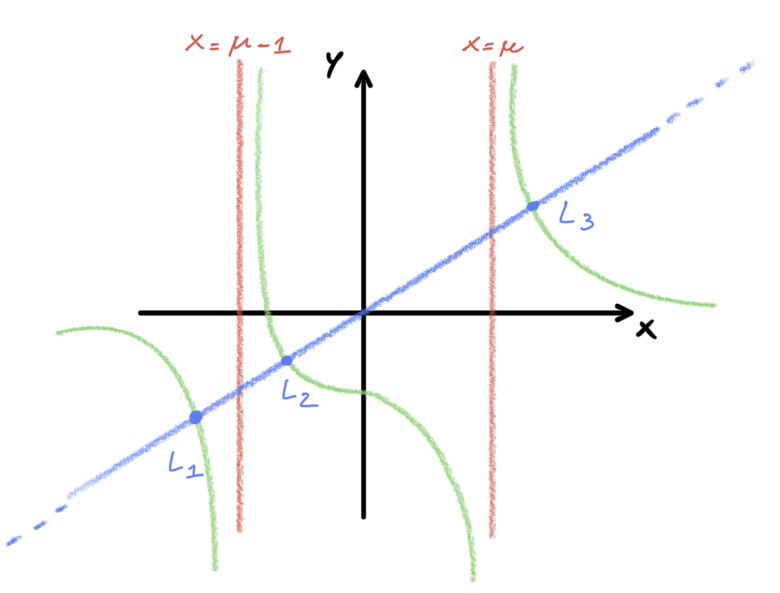
\includegraphics[scale = 0.3]{solution}	
\centering
\vspace{0.1in}
\end{figure}

\begin{itemize}
	\item Nella posizione L2 si ha che il corpo \`{e} attratto da entrambi gli altri due pianeti e dunque \`{e} in equilibrio.
	\item L1 ed L3 compaiono poich\`{e} il sistema \`{e} in rotazione. Anche se il corpo \`{e} attratto dal pianeti pi\`{u} vicino essendo il sistema di riferimento non inerziale si ha la forza apparente centrifuga.
\end{itemize}
I 3 punti di equilibrio dal punto di vista di Lyapunov sono instabili ed \`{e} applicabile il primo teorema.
Gli altri punti di equilibrio dati dal sistema (5.168) sono dati da 
\begin{equation}
\left\{\begin{array}{l}
x\left[1-\left(\frac{1-\mu}{r_1^3}+\frac{\mu}{r_2^3}\right)\right]+\mu(1-\mu)\left[\frac{1}{r_1^3}-\frac{1}{r_2{ }^3}\right]=0 \\
\left[1-\left(\frac{(1-\mu)}{r_1^3}+\frac{\mu}{r_2^3}\right)\right]=0
\end{array}\right.
\end{equation}
dunque si dalla prima equazione la condizione 
 
\begin{equation}
\left\{\begin{array}{l}
r_1 = r_2 =r \\
\left[1-\left(\frac{(1-\mu)}{r_1^3}+\frac{\mu}{r_2^3}\right)\right]=0
\end{array}\right.
\end{equation}
e risolvendo la seconda si ha che 
\begin{equation*}
	1-\frac{(1-\mu)}{r^3}-\frac{\mu}{r^3}=0 \quad \Rightarrow \quad 1-\frac{1}{r^3} = 0 \quad \Rightarrow r =1
\end{equation*}
che definisce la distanza tra i due pianeti principali. In questo modo determiniamo altri due punti di equilibrio L4,L5.
 
\begin{figure}[ht]
\vspace{0.1in}
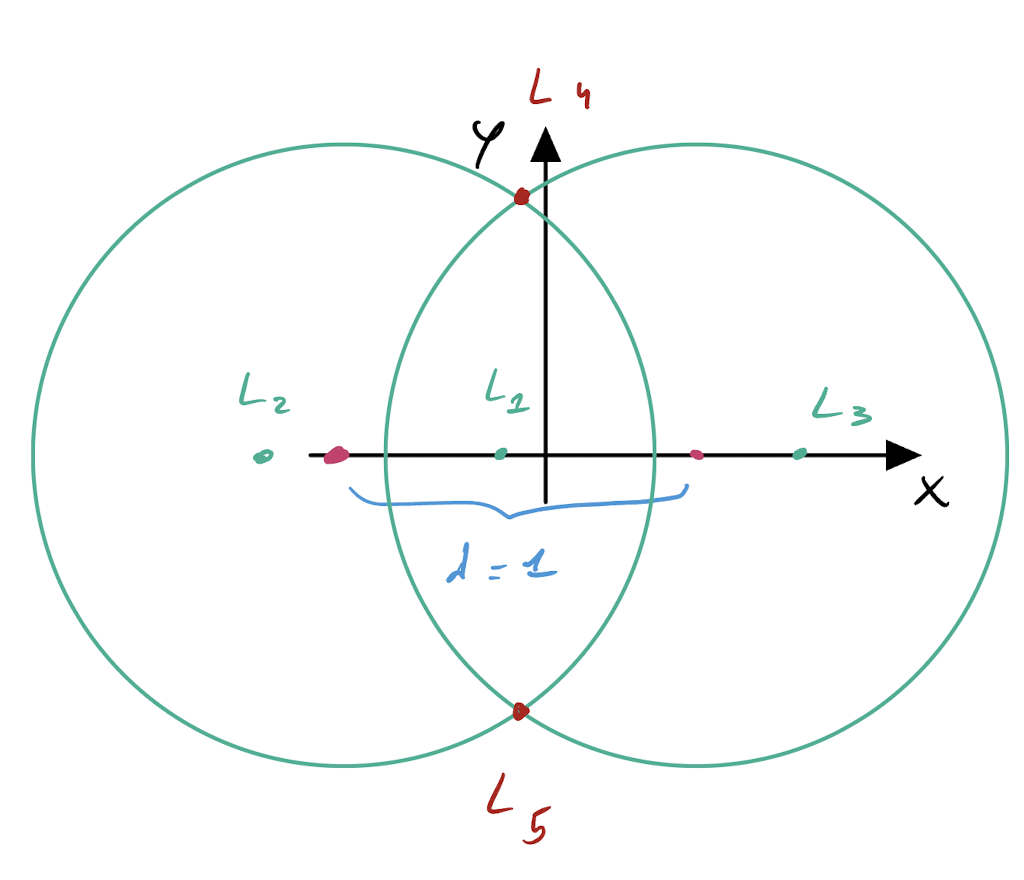
\includegraphics[scale = 0.4]{solo2}	
\centering
\vspace{0.1in}
\end{figure}
Dal primo teorema di Lyapunov si ha i punti L1,L2 ed L3 sono punti di equilibrio instabile, mentre per L4 e L5 esiste un valore critico della massa ridotta $\mu^{*} = \frac{m_2}{M} \approx 0,039$ dove se $\mu > \mu^{*}$ i due punti sono di equilibrio stabile e instabili altrimenti. I punti L1,L2 ed L3 hanno un tipo d'instabilit\`{a} simile a quella di un punto di massimo per un potenziale quartico. Infatti \`{e} possibile ottenere orbite quasi periodiche attorno al punto d'insabilit\`{a}.


